\documentclass[a4paper, 12pt]{article}
% packages
\usepackage{amssymb}
\usepackage[fleqn]{mathtools}
\usepackage{tikz}
\usepackage{enumerate}
\usepackage{bussproofs}
\usepackage{xcolor}
\usepackage[margin=1.3cm]{geometry}
\usepackage{logicproof}
\usepackage{diagbox}
\usepackage{listings}
\usepackage{graphicx}
\usepackage{lstautogobble}
\usepackage{hyperref}
\usetikzlibrary{arrows, shapes.gates.logic.US, circuits.logic.US, calc, automata, positioning}

\catcode`~=\active
\def~#1~{\texttt{#1}}

% code listing
\lstdefinestyle{main}{
    numberstyle=\tiny,
    breaklines=true,
    showspaces=false,
    showstringspaces=false,
    tabsize=2,
    numbers=left,
    basicstyle=\ttfamily,
    columns=fixed,
    fontadjust=true,
    basewidth=0.5em,
    autogobble,
    xleftmargin=3.0ex,
    mathescape=true,
}
\newcommand{\dollar}{\mbox{\textdollar}} %
\lstset{style=main}

% augmented matrix
\makeatletter
\renewcommand*\env@matrix[1][*\c@MaxMatrixCols c]{%
\hskip -\arraycolsep
\let\@ifnextchar\new@ifnextchar
\array{#1}}
\makeatother

% ceiling / floor
\DeclarePairedDelimiter{\ceil}{\lceil}{\rceil}
\DeclarePairedDelimiter{\floor}{\lfloor}{\rfloor}

% custom commands
\newcommand{\indefint}[2]{\int #1 \, \mathrm{d}#2}
\newcommand{\defint}[4]{\int_{#1}^{#2} #3 \, \mathrm{d}#4}
\newcommand{\dif}[2]{\frac{\mathrm{d}#1}{\mathrm{d}#2}}
\newcommand{\limit}[2]{\displaystyle{\lim_{#1 \to #2}}}
\newcommand{\summation}[3]{\sum\limits_{#1}^{#2} #3}
\newcommand{\intbracket}[3]{\left[#3\right]_{#1}^{#2}}

\newcommand{\powerset}[0]{\wp}
\renewcommand{\emptyset}[0]{\varnothing}

\newcommand{\unaryproof}[2]{\AxiomC{#1} \UnaryInfC{#2} \DisplayProof}
\newcommand{\binaryproof}[3]{\AxiomC{#1} \AxiomC{#2} \BinaryInfC{#3} \DisplayProof}
\newcommand{\trinaryproof}[4]{\AxiomC{#1} \AxiomC{#2} \AxiomC{#3} \TrinaryInfC{#4} \DisplayProof}

% no indent
\setlength\parindent{0pt}

% reasoning proofs
\usepackage{ltablex}
\usepackage{environ}
\keepXColumns
\NewEnviron{reasoning}{
    \begin{tabularx}{\textwidth}{rlX}
        \BODY
    \end{tabularx}
}
\newcommand{\proofline}[3]{$(#1)$ & $#2$ & \hfill #3 \smallskip \\}
\newcommand{\proofarbitrary}[1]{& take arbitrary $#1$ \smallskip \\}
\newcommand{\prooftext}[1]{\multicolumn{3}{l}{#1} \smallskip \\}
\newcommand{\proofmath}[3]{$#1$ & = $#2$ & \hfill #3 \smallskip \\}
\newcommand{\prooftherefore}[1]{& $\therefore #1$ \smallskip \\}
\newcommand{\proofbc}[0]{\prooftext{\textbf{Base Case}}}
\newcommand{\proofis}[0]{\prooftext{\textbf{Inductive Step}}}

% actual document
\begin{document}
    \section*{CO113 - Architecture}
        \subsection*{Prelude}
            The content discussed here is part of CO113 - Architecture (Computing MEng); taught by Wayne Luk, and Jana Giceva, in Imperial College London during the academic year 2018/19. The notes are written for my personal use, and have no guarantee of being correct (although I hope it is, for my own sake). This should be used in conjunction with the lecture slides, \href{https://www.youtube.com/playlist?list=PL0oekSefhQVJdk0hSRu6sZ2teWM740NtL}{\textit{The Hardware/Software Interface Class by Luis Ceze and Gaetano Borriello}} on YouTube, and \textit{Computer Organization and Design : The Hardware / Software Interface (Fifth Edition)} (chapters 1 to 4, and appendices B, and D), by Patterson, D., and Hennessy, J.
            \medskip

            The second part of the course seems to be covered in sufficient detail by the YouTube playlist, which is where the majority of the information in these notes will come from.
        \subsection*{Lecture 1 \hfill P\&H 62-120}
            Computer architecture is a combination of ISA (instruction set architecture), and machine organisation. We can see the ISA as an interface between the high level software, and the capabilities of the physical hardware components.The benefit of having the ISA is that a piece of software can be compiled into an instruction set, and then be reused on different hardware. For example, near identical versions of the x86 instruction set are used in Intel, and AMD chips despite the two having drastically different internal designs. On the other hand, microarchitecture, or computer organisation, is the the way a given ISA is implemented in a particular processor. This comes with the additional benefit that code doesn't need to be reimplemented even if there is a drastic change in the future for the microarchitecture / machine organisation.
            \medskip

            There are two design approaches, both of which have their benefits, and drawbacks;
            \begin{itemize}
                \itemsep0em
                \item Complex Instruction Set Computers (CISC)
                    \subitem The programs run on this design are closer to the high-level languages that we program in; which means that the compilers used are simpler. This is possible due to the decreasing size of transistors, and thus the increased number of gates on a chip. Programs on this instruction set tend to be smaller, as code can be represented in fewer instructions, thus saving storage.
                \item Reduced Instruction Set Computers (RISC)
                    \subitem On the other hand, the programs running on this instruction set are closer to machine code, due to the smaller range of instructions. A more powerful, better optimised, compiler will be required. Additionally, the programs here are faster, since they have simpler instructions - but they may require more instructions to achieve what a CISC can do in one, thus there may be a trade-off. It's also easier to build a chip with less instructions, which leads to lower development costs. Due to the smaller physical size of the chips, we can not only fit multiple chips together, but also use the space for memory, since accessing memory outside of the chip is very slow (compared to the high-speed registers nearby).
            \end{itemize}
            In this course, we will be working mostly on a MIPS processor. Generally, the instructions consist of an opcode, which is what it does, and an operand (which includes the registers, memory locations, and data). This should be fairly similar to the very end of \textbf{CO112 - Hardware}. The design principle for RISCs is that the processor should have good performance, and be relatively simple to implement. In MIPS, there are 3 main types of instructions; R (register), I (immediate), and J (jump), all of which have a fixed size of 32 bits.
            \medskip

            MIPS is representative of modern RISC architectures, and has 32 registers, each being able to store 32-bit data. The registers are named \$0..\$31, with \$0 being typically wired to ground (logic 0), and the others being used for general-purpose storage. MIPS is known as a register-register, or load-store architecture, which means that there are two different sets of instructions; one that is extremely fast, and works between registers, and another set working with memory access, which tends to be slower. The goal is to minimise memory access, as accessing data from memory tends to be much slower than accessing memory located in the registers on the chip. Here are some examples of these instructions;
            \begin{itemize}
                \itemsep0em
                \item register-register
                    \subitem \texttt{add \$1, \$2, \$3} \hfill reg1 = reg2 + reg3
                \item load-store
                    \subitem \texttt{lw \$8, Astart(\$19)} \hfill reg8 = M[Astart + reg19]
            \end{itemize}
            R-type instructions can be used for arithmetic, comparisons, logical operations, etc. and have a general format as follows (the example describes \texttt{add \$8, \$17, \$18}). It's important to note that we have an additional 6 bits at the end for the function, since having a 6-bit opcode only leaves us 64 ($2^6$) instructions, which is quite limited even for a RISC instruction set. In addition, the shift amount specifies the amount of bits to shift, if it was a shift instruction, however it's redundant in this case;
            \begin{center}
                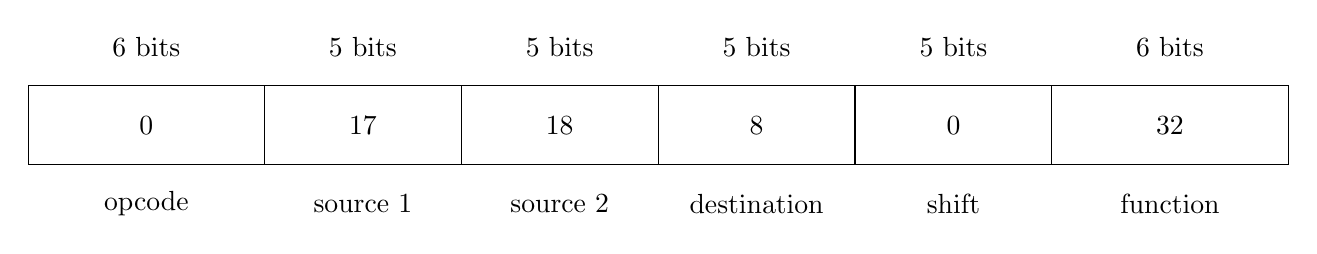
\begin{tikzpicture}
                    \draw
                    (0, 0) -- (16, 0) -- (16, -1) -- (0, -1) -- cycle;

                    \draw
                    (3, 0) -- (3, -1)
                    (5.5, 0) -- (5.5, -1)
                    (8, 0) -- (8, -1)
                    (10.5, 0) -- (10.5, -1)
                    (13, 0) -- (13, -1);

                    \node[] () at (1.5, -0.5) {0};
                    \node[] () at (4.25, -0.5) {17};
                    \node[] () at (6.75, -0.5) {18};
                    \node[] () at (9.25, -0.5) {8};
                    \node[] () at (11.75, -0.5) {0};
                    \node[] () at (14.5, -0.5) {32};

                    \node[] () at (1.5, 0.5) {6 bits};
                    \node[] () at (4.25, 0.5) {5 bits};
                    \node[] () at (6.75, 0.5) {5 bits};
                    \node[] () at (9.25, 0.5) {5 bits};
                    \node[] () at (11.75, 0.5) {5 bits};
                    \node[] () at (14.5, 0.5) {6 bits};

                    \node[] () at (1.5, -1.5) {opcode};
                    \node[] () at (4.25, -1.5) {source 1};
                    \node[] () at (6.75, -1.5) {source 2};
                    \node[] () at (9.25, -1.5) {destination};
                    \node[] () at (11.75, -1.5) {shift};
                    \node[] () at (14.5, -1.5) {function};
                \end{tikzpicture}
            \end{center}
            I-type instructions are used for memory access, conditional branching, or arithmetic with constants. An example of doing addition with constants is \texttt{addi \$1, \$2, 100}, which does reg1 = reg2 + 100. The example displayed below is \texttt{lw \$8, Astart(\$19)}, which does reg8 = M[Astart + reg19].
            \begin{center}
                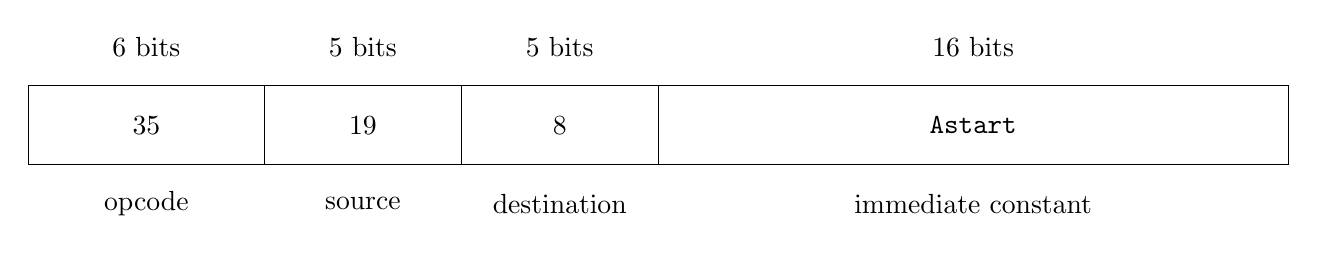
\begin{tikzpicture}
                    \draw
                    (0, 0) -- (16, 0) -- (16, -1) -- (0, -1) -- cycle;

                    \draw
                    (3, 0) -- (3, -1)
                    (5.5, 0) -- (5.5, -1)
                    (8, 0) -- (8, -1);

                    \node[] () at (1.5, -0.5) {35};
                    \node[] () at (4.25, -0.5) {19};
                    \node[] () at (6.75, -0.5) {8};
                    \node[] () at (12, -0.5) {\texttt{Astart}};

                    \node[] () at (1.5, 0.5) {6 bits};
                    \node[] () at (4.25, 0.5) {5 bits};
                    \node[] () at (6.75, 0.5) {5 bits};
                    \node[] () at (12, 0.5) {16 bits};

                    \node[] () at (1.5, -1.5) {opcode};
                    \node[] () at (4.25, -1.5) {source};
                    \node[] () at (6.75, -1.5) {destination};
                    \node[] () at (12, -1.5) {immediate constant};
                \end{tikzpicture}
            \end{center}
            Finally J-type instructions are jump to instructions in memory, for example, \texttt{j 1236} would be an unconditional jump to the instruction at address 1236. An unconditional jump has the following format;
            \begin{center}
                \begin{tikzpicture}
                    \draw
                    (0, 0) -- (16, 0) -- (16, -1) -- (0, -1) -- cycle;

                    \draw
                    (3, 0) -- (3, -1);

                    \node[] () at (1.5, -0.5) {2};
                    \node[] () at (9.5, -0.5) {1236};

                    \node[] () at (1.5, 0.5) {6 bits};
                    \node[] () at (9.5, 0.5) {26 bits};

                    \node[] () at (1.5, -1.5) {opcode};
                    \node[] () at (9.5, -1.5) {memory location};
                \end{tikzpicture}
            \end{center}
            However, we can also have jump instructions, which are I-type, or R-type, for example \texttt{bne \$19, \$20, Label} is an I-type instruction, where the program jumps to \texttt{Label} if registers 19, and 20 aren't equal. An R-type example would be \texttt{jr \$ra}, where it jumps to the address in register ra.

            Consider the following program, and its equivalent in machine code, the registers are labeled in alphabetical order (reg16 = f, reg20 = j, etc);
            \begin{lstlisting}
                if (i == j) {
                  f = g + h;
                } else {
                  f = g - h;
                }

                      bne $\dollar$19, $\dollar$20, Else # if i $\neq$ j goto Else
                      add $\dollar$16, $\dollar$17, $\dollar$18     # f = g + h
                      j   Exit           # goto Exit
                Else: sub $\dollar$16, $\dollar$17, $\dollar$18     # f = g - h
                Exit:
            \end{lstlisting}
            Since we only have two types of conditional branches, \texttt{bne}, and \texttt{beq}, we need \texttt{slt}, which does the following - \texttt{slt \$1, \$16, \$17}, if reg16 $<$ reg17, then it sets reg1 to 1, otherwise it's set to 0. Then, we can use \texttt{bne}, with \texttt{\$0}, since reg0 is always set to logic 0.
        \subsection*{Lecture 2 \hfill P\&H 28-53}
            One of the questions raised in this lecture is the following; "Is a 20\% cheaper processor, with the same performance good enough?". While this may seem straightforward, from a consumer's perspective, it's important to note that a consumer has instant gratification from buying a product, but developing one would take time. In this time, competitors are also trying to improve on their product, and as such you can't just know the price, and performance of a competitor's product \textbf{now}, but you also need to predict the improvement.
            \medskip

            CPI is the \textbf{average} number of clock cycles required per instruction. Note that it's the average, because some instructions may take more cycles to complete. For a given program $P$, we can get the number of cycles required for $P$ by doing the number of instructions in $P$, multiplied by the CPI. The execution time for $P$ is the number of cycles in $P$, multiplied by the clock cycle time (which is $\frac{1}{\text{clock speed}}$). Assuming that for a set of programs $P_1$, ..., $P_n$, the workload is equal, we can calculate the average execution time for the set by taking the mean of the execution times.
            \subsubsection*{Example}
                Consider two machines, $M_1$, and $M_2$, which implement the same instruction set that has 2 classes of instructions; $A$, and $B$. The CPI for $M_1$ on class $A$ is $A_1$, $B$, is $B_1$, and the same for $M_2$. The clock speed of $M_1$ is $C_1$ MHz, and similar for $M_2$. If we were to compare their peak and average performance of $N$ instructions, half of which are of class $A$, and the other half of class $B$, we'd need to find the ratio of execution times.
                \medskip

                In order to find the peak performance of $N$ instructions for $M_1$ (let it be $P_{P1}$), we take the clock cycle time (which is $\frac{1}{C_1}$, multiply it by the number of instructions $N$, miltiply it by the \textbf{minimum} CPI for $M_1$ (which would be min($A_1$, $B_1$)), we'd get $\frac{N(\text{min}(A_1, B_1))}{C_1}$. To compare the two, we take $\frac{P_{P1}}{P_{P2}} = \frac{\text{min}(A_1, B_1) \cdot C_2}{\text{min}(A_2, B_2) \cdot C_1}$.
                \medskip

                We do a similar process for finding the average performance, let it be $P_{A1}$, but instead of multiplying it by the minimum CPI, we take the average, hence we multiply by $\frac{A_1 + B1}{2}$. To compare the two, we take $\frac{P_{A1}}{P_{A2}} = \frac{(A_1 + B_1) \cdot C_2}{(A_2 + B_2) \cdot C_1}$.
                \medskip

                Our goal is to minimize the execution time, which is to minimise $\text{instruction count} \times \text{CPI} \times \text{cycle time}$. Consider this example, comparing SUN 68000, and their newer SUN RISC. In the RISC device, there are 25\% more instructions, and the cycle time is 50\% longer. However, the CPI is much lower, as the instructions are simpler, thus requiring less cycles. The price has increased, but the performance has doubled.
                \begin{center}
                    \begin{tabular}{l|l|l}
                        & SUN 68000 & SUN RISC \\
                        \hline
                        Instruction Count Ratio & 1.0 & 1.25 \\
                        Cycle time & 40ns & 60ns \\
                        CPI & 5.0 - 7.0 & 1.3 - 1.7 \\
                        Execution Time Ratio & 2 & 1 \\
                        Price Ratio & 1 & 1.1 - 1.2
                    \end{tabular}
                \end{center}
                The processor time is measured by the seconds per program, which is calculated as follows; $\frac{\text{time}}{\text{program}} = \frac{\text{instructions}}{\text{program}} \cdot \frac{\text{cycles}}{\text{instruction}} \cdot \frac{\text{time}}{\text{cycle}}$.
            \subsubsection*{RISC}
                Regarding the principles of RISC instruction set design, the common cases should be optimised, thus reducing the CPI. A small number of general purpose registers (32 in MIPS), simplifies things, and allows the design to be more adaptable to new technologies. The smaller chip size allows for a higher yield, thus reducing the cost of production. On the other hand, the lower number of instructions increases the code size, and smarter compilers are needed, since the instructions are further away from the software level than with a CISC instruction set.
            \subsubsection*{Performance Trends}
                In 2004, the trend in power usage hit a peak, due to heat not being able to be removed from the chip at a reasonable rate. The voltage also cannot be reduced further, which is why the trends seemed to have become flat. $P = C \cdot V^2 \cdot F$, where $P$ is power, $C$ is capacitive load, $V$ is voltage, and $F$ is frequency.
                \medskip

                Other than just increasing clock speed, performance can be increased in other ways; including faster local storage, concurrent execution, and newer technologies. Implementning on-chip caches allows for faster execution due to the faster memory closer to the chip, which would be a significant improvement compared to fetching from RAM. Concurrent execution can be achieved by multiple function units (super scalar), a pipeline execution, or multiple instruction streams (multi-threading). Newer technologies, such as GPUs can also be used for specialised loads.
            \subsubsection*{Benchmarking}
                There are a number of ways of benchmarking, each with their benefits, and drawbacks as follows;
                \begin{center}
                    \begin{tabular}{l|l|l}
                        method & pros & cons \\
                        \hline
                        actual target workload & representative & very specific, not portable \\
                        & & difficult to measure \\
                        & & hard to identify problems \\
                        \hline
                        full benchmarks & portable & less representative \\
                        & widespread usage & \\
                        \hline
                        kernel benchmarks & easy to use & peak is not representative \\
                        & used early in design cycle & \\
                        & identify peak performance &
                    \end{tabular}
                \end{center}
        \subsection*{Lecture 3}
            Considering the software side of parallelism; we have parallel requests, parallel threads, parallel instructions, and parallel data. Parallel threads schedule tasks; for example if you have an instruction that takes longer to process since it has to read from main memory, or wait for another resource, another task can be scheduled to run during this time. Since a processor core has multiple functional units, instructions can be arranged in a pipeline, where different stages are processed at the same time. Finally, data can be parallelised, as each item of data can contain multiple chunks of data, each of which can be operated on separately.
            \medskip

            In MIPS, we have 3 different types of addressing;
            \begin{itemize}
                \itemsep0em
                \item register addressing \hfill accessing the data in registers
                \item immediate addressing \hfill data is contained within the instruction (I-type)
                \item base addressing \hfill accessing data in memory with load/store instructions
                \item PC-relative addressing \hfill replaces the register with the program counter (in the I-type load)
            \end{itemize}
            We can classify architectures by how they address temporary storage. Here we cover three main types - all of which are operating on the same code; which is \texttt{C = A + B};
            \begin{itemize}
                \itemsep0em
                \item stack \hfill operands are implicitly specified at the top of the stack
                    \subitem \texttt{push A; push B; add; pop C}
                    \subitem this adds the top pair of items on the stack
                    \subitem pros: it has a simple evaluation model, and the code is dense
                    \subitem cons: this model is less flexible, has no random access, and is slow if the stack is in memory
                \item accumulator \hfill one operand in the accumulator
                    \subitem \texttt{load A; add B; store C}
                    \subitem this adds the accumulator, and the data in memory
                    \subitem pros: there is minimal internal storage, and has short instructions
                    \subitem cons: there is frequent memory access, therefore it is slower
                \item register \hfill we explicitly state the operands
                    \subitem \texttt{load R1 A; add R2, R1, B; store C, R2}
                    \subitem this simply adds two registers
                    \subitem pros: this is the general model for code generation, and has faster register access
                    \subitem cons: this requires you to name all the operands, and also has longer instructions
            \end{itemize}
            Most modern architectures are register based, as it's still faster, as there is less memory traffic, as well as the code being denser. At the start, the first computers used single accumulators, as memory was still expensive, and therefore registers had to be used sparingly.
            \subsubsection*{Amdahl's Law}
                When some instructions are used frequently, and are normally expensive to compute, there are three possible approaches (for example, repeatedly calculating $x^2 + y^2$);
                \begin{enumerate}[1.]
                    \itemsep0em
                    \item add instruciton, accumulator, or load-store
                    \item add, and square instructions, accumulator, or load-store
                    \item custom sumsq instruction, with a dedicated circuit
                \end{enumerate}
                However, this is not always beneficial (or worth the additional cost, and time). For example, consider a program that takes $T_\text{old}$ time to run, and a fraction of the code $\alpha$ can be sped up $\beta$ times. Now, we can calculate the new runtime of the code as $T_\text{new} = \alpha \frac{T_\text{old}}{\beta} + (1 - \alpha)T_\text{old}$. Let's have an example, wehre 90\% of the code can be sped up 100 times, such that $\alpha = 0.9$, and $\beta = 100$. By running this calculation, we can say that $T_\text{old} \approx 9.17 \cdot T_\text{new}$ - the code is less than 10 times faster.
        \subsection*{Lecture 4}
            There are two ways of representing negative numbers in binary, two's complement, and sign-and-magnitude. When we use sign-and-magnitude, it may be more intuitive for us, but for a computer to do addition on it may be problematic as we can easily lose (or gain) the sign bit. On the other hand, two's complement is more complex, but allows for easier operations. For example, you can repeat the most significant bit (e.g. $\texttt{10}_\text{2C} = \texttt{111110}_\text{2C} = -2_\text{Dec}$)
            \medskip

            The layout of a MIPS ALU is similar to the basic one covered in \textbf{CO112}, as in, it has separate units for bit-wise AND, bit-wise OR, addition, etc. and also does the all the operations, then selects one based on the input. Similarly, it also uses the same slash notation to denote $n$ lines being connected. On the gate level, it's important to remember the following;
            \begin{center}
                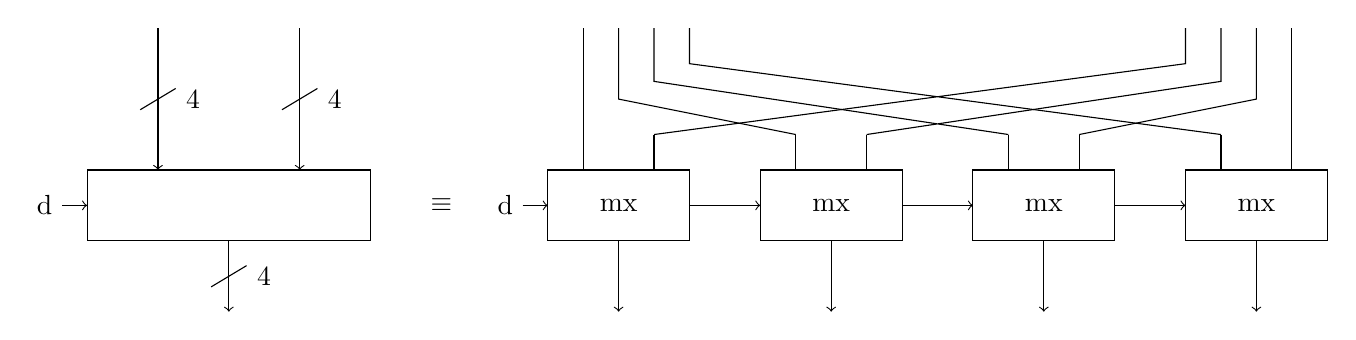
\begin{tikzpicture}[x=0.9cm, y=0.9cm]
                    \node[] (d) at (-0.6, -0.5) {d};
                    \draw
                    (0, 0) -- (4, 0) -- (4, -1) -- (0, -1) -- cycle
                    (1, 2) edge[->] (1, 0)
                    (3, 2) edge[->] (3, 0)
                    (2, -1) edge[->] (2, -2)
                    (d) edge[->] (0, -0.5);

                    \node[] (i1) at (1, 1) {};
                    \node[] (i2) at (3, 1) {};
                    \node[] (o) at (2, -1.5) {};

                    \draw
                    ($(i1) + (-0.25, -0.15)$) edge[right] node{\ \ 4} ($(i1) + (0.25, 0.15)$)
                    ($(i2) + (-0.25, -0.15)$) edge[right] node{\ \ 4} ($(i2) + (0.25, 0.15)$)
                    ($(o) + (-0.25, -0.15)$) edge[right] node{\ \ 4} ($(o) + (0.25, 0.15)$);

                    \node[] (d2) at (5.9, -0.5) {d};
                    \foreach \x in {0,...,3} {
                        \draw
                        (6.5 + 3*\x, 0) -- (8.5 + 3*\x, 0) -- (8.5 + 3*\x, -1) -- (6.5 + 3*\x, -1) -- cycle
                        (7.5 + 3*\x, -1) edge[->] (7.5 + 3*\x, -2)
                        (7 + 3*\x, 0) -- (7 + 3*\x, 0.5)
                        (8 + 3*\x, 0) -- (8 + 3*\x, 0.5);

                        \node[] () at (7.5 + 3*\x, -0.5) {mx};

                        \draw
                        (7 + 0.5*\x, 2) -- (7 + 0.5*\x, 0.75 + 0.25*\x) -- (7 + 3*\x, 0.5)
                        (17 - 0.5*\x, 2) -- (17 - 0.5*\x, 0.75 + 0.25*\x) -- (17 - 3*\x, 0.5);
                    }

                    \draw
                    (d2) edge[->] (6.5, -0.5)
                    (8.5, -0.5) edge[->] (9.5, -0.5)
                    (11.5, -0.5) edge[->] (12.5, -0.5)
                    (14.5, -0.5) edge[->] (15.5, -0.5);

                    \node[] () at (5, -0.5) {$\equiv$};
                \end{tikzpicture}
            \end{center}
            A similar diagram can also be used for the ripple carry adder, which joins $n$ full adders, to create an $n$-bit ripple adder.
            \begin{center}
                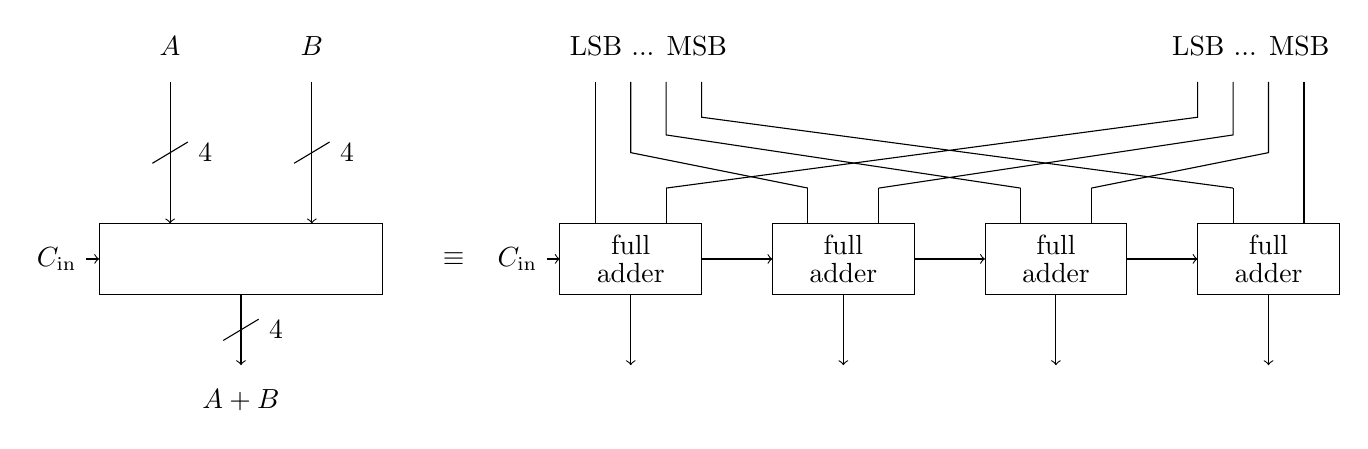
\begin{tikzpicture}[x=0.9cm, y=0.9cm]
                    \node[] (d) at (-0.6, -0.5) {$C_\text{in}$};
                    \draw
                    (0, 0) -- (4, 0) -- (4, -1) -- (0, -1) -- cycle
                    (1, 2) edge[->] (1, 0)
                    (3, 2) edge[->] (3, 0)
                    (2, -1) edge[->] (2, -2)
                    (d) edge[->] (0, -0.5);

                    \node[] (i1) at (1, 1) {};
                    \node[] (i2) at (3, 1) {};
                    \node[] (o) at (2, -1.5) {};

                    \draw
                    ($(i1) + (-0.25, -0.15)$) edge[right] node{\ \ 4} ($(i1) + (0.25, 0.15)$)
                    ($(i2) + (-0.25, -0.15)$) edge[right] node{\ \ 4} ($(i2) + (0.25, 0.15)$)
                    ($(o) + (-0.25, -0.15)$) edge[right] node{\ \ 4} ($(o) + (0.25, 0.15)$);

                    \node[] (d2) at (5.9, -0.5) {$C_\text{in}$};
                    \foreach \x in {0,...,3} {
                        \draw
                        (6.5 + 3*\x, 0) -- (8.5 + 3*\x, 0) -- (8.5 + 3*\x, -1) -- (6.5 + 3*\x, -1) -- cycle
                        (7.5 + 3*\x, -1) edge[->] (7.5 + 3*\x, -2)
                        (7 + 3*\x, 0) -- (7 + 3*\x, 0.5)
                        (8 + 3*\x, 0) -- (8 + 3*\x, 0.5);

                        \node[] () at (7.5 + 3*\x, -0.5) {\shortstack{full\\adder}};

                        \draw
                        (7 + 0.5*\x, 2) -- (7 + 0.5*\x, 0.75 + 0.25*\x) -- (7 + 3*\x, 0.5)
                        (17 - 0.5*\x, 2) -- (17 - 0.5*\x, 0.75 + 0.25*\x) -- (17 - 3*\x, 0.5);
                    }

                    \node[] () at (7.75, 2.5) {LSB ... MSB};
                    \node[] () at (16.25, 2.5) {LSB ... MSB};
                    \node[] () at (1, 2.5) {$A$};
                    \node[] () at (3, 2.5) {$B$};
                    \node[] () at (2, -2.5) {$A+B$};
                    \draw
                    (d2) edge[->] (6.5, -0.5)
                    (8.5, -0.5) edge[->] (9.5, -0.5)
                    (11.5, -0.5) edge[->] (12.5, -0.5)
                    (14.5, -0.5) edge[->] (15.5, -0.5);

                    \node[] () at (5, -0.5) {$\equiv$};
                \end{tikzpicture}
            \end{center}
            With this full adder, we are able to use this as as subtractor. For example, when working with $A - B$; take the ones complement of $B$ (which is inverting $B$ bitwise), and add it to $A$, and setting $C_\text{in}$ to 1. Bitwise inversion is done with an XOR, when the otger input is 1. Other important circuits found in our ALU, are the AOR (which is shown below);
            \begin{center}
                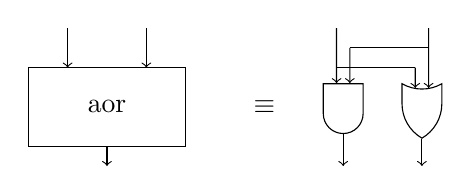
\begin{tikzpicture}
                    \node[] () at (1, 0) {aor};
                    \node[] () at (3, 0) {$\equiv$};

                    \draw
                    (0, 0.5) -- (2, 0.5) -- (2, -0.5) -- (0, -0.5) -- cycle
                    (0.5, 1) edge[->] (0.5, 0.5)
                    (1.5, 1) edge[->] (1.5, 0.5)
                    (1, -0.5) edge[->] (1, -0.75);

                    \node[and gate US, draw, logic gate inputs=nn, rotate=-90] (and) at (4, 0) {};
                    \node[or gate US, draw, logic gate inputs=nn, rotate=-90] (or) at (5, 0) {};

                    \draw
                    (4 - 0.085, 1) edge[->] (and.input 2)
                    (5 + 0.085, 1) edge[->] (or.input 1)
                    (4 - 0.085, 0.5) -- (5 - 0.085, 0.5) edge[->] (or.input 2)
                    (5 + 0.085, 0.75) -- (4+ 0.085, 0.75) edge[->] (and.input 1)
                    (and.output) edge[->] (4, -0.75)
                    (or.output) edge[->] (5, -0.75);
                \end{tikzpicture}
            \end{center}
            This can then be combined with a single full adder block, to create AFA;
            \begin{center}
                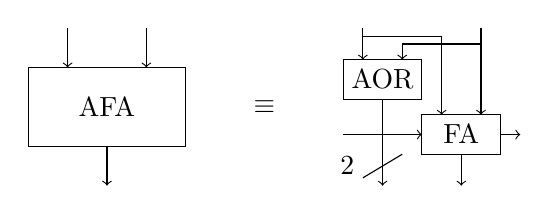
\begin{tikzpicture}
                    \node[] () at (1, 0) {AFA};
                    \node[] () at (3, 0) {$\equiv$};

                    \draw
                    (0, 0.5) -- (2, 0.5) -- (2, -0.5) -- (0, -0.5) -- cycle
                    (0.5, 1) edge[->] (0.5, 0.5)
                    (1.5, 1) edge[->] (1.5, 0.5)
                    (1, -0.5) edge[->] (1, -1);

                    \node[] () at (4.5, 0.35) {AOR};
                    \node[] () at (5.5, -0.35) {FA};
                    \node[] (o) at (4.5, -0.75) {};

                    \draw
                    (4, 0.6) -- (5, 0.6) -- (5, 0.1) -- (4, 0.1) -- cycle
                    (5, -0.1) -- (6, -0.1) -- (6, -0.6) -- (5, -0.6) -- cycle
                    (4.25, 1) edge[->] (4.25, 0.6)
                    (5.75, 1) edge[->] (5.75, -0.1)
                    (4.25, 0.9) -- (5.25, 0.9) edge[->] (5.25, -0.1)
                    (5.75, 0.8) -- (4.75, 0.8) edge[->] (4.75, 0.6)
                    (4.5, 0.1) edge[->] (4.5, -1)
                    (5.5, -0.6) edge[->] (5.5, -1)
                    (4, -0.35) edge[->] (5, -0.35)
                    (6, -0.35) edge[->] (6.25, -0.35)
                    ($(o) + (-0.25, -0.15)$) edge[left] node{2\ \ \ } ($(o) + (0.25, 0.15)$);
                \end{tikzpicture}
            \end{center}
            With these components, we can build our first ALU block;
            \begin{center}
                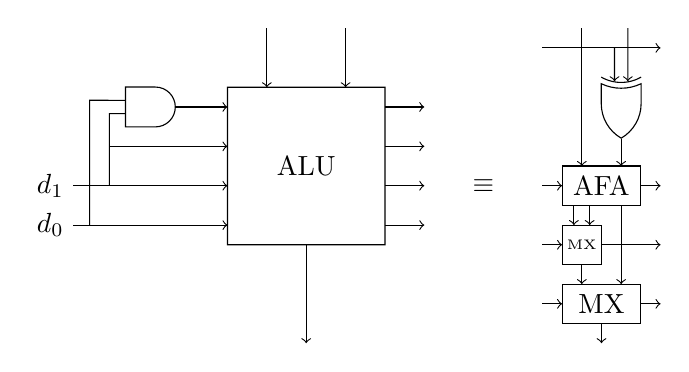
\begin{tikzpicture}
                    \node[and gate US, draw, logic gate inputs=nn] (and) at (0, 0) {};
                    \node[] () at (2, -0.75) {ALU};
                    \node[] (d0) at (-1.25, -1.5) {$d_0$};
                    \node[] (d1) at (-1.25, -1) {$d_1$};
                    \draw
                    (1, 0.25) -- (3, 0.25) -- (3, -1.75) -- (1, -1.75) -- cycle
                    (and.output) edge[->] (1, 0)
                    (-0.5, -0.5) edge[->] (1, -0.5)
                    (d1) edge[->] (1, -1)
                    (d0) edge[->] (1, -1.5)
                    (-0.75, -1.5) -- (-0.75, 0.085) -- (and.input 1)
                    (-0.5, -1) -- (-0.5, -0.085) -- (and.input 2)
                    (1.5, 1) edge[->] (1.5, 0.25)
                    (2.5, 1) edge[->] (2.5, 0.25)
                    (2, -1.75) edge[->] (2, -3)
                    \foreach \x in {0,...,3} {
                        (3, -1.5 + 0.5*\x) edge[->] (3.5, -1.5 + 0.5*\x)
                    };

                    \node[] () at (5.75, -1) {AFA};
                    \node[] () at (5.5, -1.75) {\tiny MX};
                    \node[] () at (5.75, -2.5) {MX};
                    \node[xor gate US, draw, logic gate inputs=nn, rotate=-90] (xor) at (6, 0) {};
                    \node[] () at (4.25, -1) {$\equiv$};
                    \draw
                    (5, 0.75) edge[->] (6.5, 0.75)
                    (6 - 0.085, 0.75) edge[->] (xor.input 2)
                    (6 + 0.085, 1) edge[->] (xor.input 1)
                    (5.25, -0.75) -- (6.25, -0.75) -- (6.25, -1.25) -- (5.25, -1.25) -- cycle
                    (5.25, -1.5) -- (5.75, -1.5) -- (5.75, -2) -- (5.25, -2) -- cycle
                    (5.25, -2.25) -- (6.25, -2.25) -- (6.25, -2.75) -- (5.25, -2.75) -- cycle
                    (5, -1) edge[->] (5.25, -1)
                    (5, -1.75) edge[->] (5.25, -1.75)
                    (5, -2.5) edge[->] (5.25, -2.5)
                    (6.25, -1) edge[->] (6.5, -1)
                    (5.75, -1.75) edge[->] (6.5, -1.75)
                    (6.25, -2.5) edge[->] (6.5, -2.5)
                    (xor.output) edge[->] (6, -0.75)
                    (5.5, 1) edge[->] (5.5, -0.75)
                    (5.4, -1.25) edge[->] (5.4, -1.5)
                    (5.6, -1.25) edge[->] (5.6, -1.5)
                    (5.5, -2) edge[->] (5.5, -2.25)
                    (6, -1.25) edge[->] (6, -2.25)
                    (5.75, -2.75) edge[->] (5.75, -3);
                \end{tikzpicture}
            \end{center}
            This design for the ALU has the functions $d_0d_1$, where 00 is AND, 01 is OR, 10 is addition, and 11 is subtraction. Remember that the carry is only set to 1 at the start when we're doing subtraction. The top line is also set to 1 when we're doing subtraction.
            \medskip

            The carry path is often the slowest line, as it needs to go through many gates of logic, which limits the clock rate, since clock rate $\approx \frac{1}{\text{delay of slowest path}}$, given we have an edge-triggered design, and a few other factors (from P\&H Appendix B. 11)
        \subsection*{Lecture 5 \hfill P\&H 183-196}
            \subsubsection*{Multiplication Algorithm}
                Consider the example $2 \cdot 11 = 22$, we have the multiplicand times the multiplier = product. However, to do this bitwise, we have to do the following (let $c \leftarrow n$ mean $c$ shifted $n$ bits to the left, and $b_i$ mean the $i^\text{th}$ bit of $b$);
                \begin{center}
                    \begin{tabular}{cccccccccl}
                        & & & & & 0 & 0 & 1 & 0 & multiplicand ($c$) \\
                        $\times$ & & & & & 1 & 0 & 1 & 1 & multiplier ($p$) \\
                        \hline
                        & & & & & 0 & 0 & 1 & 0 & $(c \leftarrow 0) \cdot p_0$ \\
                        & & & & 0 & 0 & 1 & 0 & & $(c \leftarrow 1) \cdot p_1$ \\
                        & & & 0 & 0 & 0 & 0 & & & $(c \leftarrow 2) \cdot p_2$ \\
                        + & & 0 & 0 & 1 & 0 & & & & $(c \leftarrow 3) \cdot p_3$ \\
                        \hline
                        & & 0 & 0 & 1 & 0 & 1 & 1 & 0 &
                    \end{tabular}
                \end{center}
                Note that the third line is all 0s, because $p_2$ is 0, and multiplication is just AND. The idea is that the product is the miltiplicand shifted succesively by 1 bit relative to the multiplier; CSAA - conditional shift and add. We only really need to shift when the bit isn't 0.
            \subsubsection*{Another Multiplication Algorithm}
                However, there are other options for multiplication algorithms, which can save silicon space; we can use a 32-bit ALU, and a 64-bit register, which stores both the product, and the multiplier initially.
                \begin{center}
                    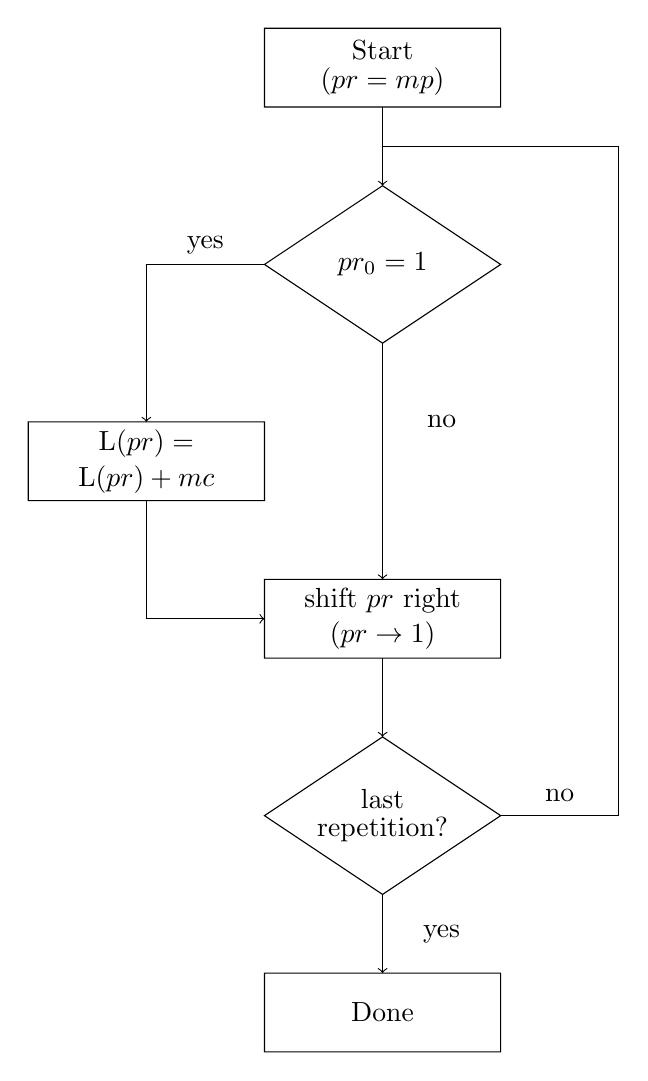
\begin{tikzpicture}[x=1.5cm, y=1cm]
                        \draw
                        (-1, 0) -- (1, 0) -- (1, -1) -- (-1, -1) -- cycle
                        (0, -2) -- (1, -3) -- (0, -4) -- (-1, -3) -- cycle
                        (-3, -5) -- (-1, -5) -- (-1, -6) -- (-3, -6) -- cycle
                        (-1, -7) -- (1, -7) -- (1, -8) -- (-1, -8) -- cycle
                        (0, -9) -- (1, -10) -- (0, -11) -- (-1, -10) -- cycle
                        (-1, -12) -- (1, -12) -- (1, -13) -- (-1, -13) -- cycle;

                        \draw
                        (0, -1) edge[->] (0, -2)
                        (-1, -3) -- (-2, -3) edge[->] (-2, -5)
                        (-2, -6) -- (-2, -7.5) edge[->] (-1, -7.5)
                        (0, -4) edge[->] (0, -7)
                        (0, -8) edge[->] (0, -9)
                        (0, -11) edge[->] (0, -12)
                        (1, -10) -- (2, -10) -- (2, -1.5) -- (0, -1.5);

                        \node[] () at (0, -0.5) {\shortstack{Start \\ $(pr = mp)$}};
                        \node[] () at (0, -3) {$pr_0 = 1$};
                        \node[] () at (-1.5, -2.75) {yes};
                        \node[] () at (0.5, -5) {no};
                        \node[] () at (-2, -5.5) {\shortstack{$\text{L}(pr) =$ \\ $\text{L}(pr) + mc$}};
                        \node[] () at (0, -7.5) {\shortstack{shift $pr$ right \\ $(pr \rightarrow 1)$}};
                        \node[] () at (0, -10) {\shortstack{last \\ repetition?}};
                        \node[] () at (0.5, -11.5) {yes};
                        \node[] () at (1.5, -9.75) {no};
                        \node[] () at (0, -12.5) {Done};
                    \end{tikzpicture}
                \end{center}
            \subsubsection*{Booth's Algorithm}
                When we have a string of repeated 1s, we can change $n$ additions into 1 addition, and 1 subtraction. As we're summing a geometric series, when we do repeated additions, such that $m + 2m + 2^2m + ... + 2^{k-1}m = -m + 2^km$. This is much easier to compute, as all we have to do is to do an arithmetic shift on $m$, and a subtraction. However, instead of checking only the LSB ($pr_0$), we also check the previous LSB, let it be $pr_{-1}$. We have the following cases, written $pr_0pr_{-1}$; 00 or 11 - we're in the middle of a string of 0s (or 1s, respectively), no action is needed, 01 - we're at the end of a string of 1s, $pr = pr + mc$ (where $mc$ is the shifted multiplicand), and 10 - we're at the start of a string of 1s, $pr = pr - mc$. Note that in my version of the slides (2018 - 2019 academic year), there is a typo on slide 15. The "corrected" version is below (this is working on $\texttt{0010}_2 \times \texttt{0110}_2$), and $mc$ is \texttt{0010}. Also note that $\text(pr)$ means the left half of the product register;
                \begin{center}
                    \begin{tabular}{c|lr|lr}
                        iteration & \multicolumn{2}{c|}{original} & \multicolumn{2}{c}{Booth's} \\
                        & step & product & step & product \\
                        \hline
                        0 & initial values & 0000 011\textbf{0} & initial values & 0000 011\textbf{0} \textbf{0} \\
                        \hline
                        1 & 1a: 0 - no operation & 0000 0110 & 1a: 00 - no operation & 0000 0110 0 \\
                        & 2: product shift right & 0000 001\textbf{1} & 2: product shift right & 0000 001\textbf{1} \textbf{0} \\
                        \hline
                        2 & 1b: 1 - $\text{L}(pr) = \text{L}(pr) + mc$ & 0010 0011 & 1c: 10 - $\text{L}(pr) = \text{L}(pr) - mc$ & 1110 0011 0 \\
                        & 2: product shift right & 0001 000\textbf{1} & 2: product shift right & 1111 000\textbf{1} \textbf{1} \\
                        \hline
                        3 & 1b: 1 - $\text{L}(pr) = \text{L}(pr) + mc$ & 0011 0001 & 1d: 11 - no operation & 1111 0001 1 \\
                        & 1: product shift right & 0001 100\textbf{0} & 2: product shift right & 1111 100\textbf{0} \textbf{1} \\
                        \hline
                        4 & 1a: 0 - no operation & 0001 1000 & 1b: 01 - $\text{L}(pr) = \text{L}(pr) + mc$ & 0001 1000 1 \\
                        & 1: product shift right & 0000 1100 & 2: product shift right & 0000 1100 0 \\
                    \end{tabular}
                \end{center}
            \subsubsection*{Division}
                This algorithm was invented by Briggs; dividend = quotient $\times$ divisor + remainder. We can work through an example of the first algorithm as follows; case 2b is when $rem < 0$, and 2a is when $rem \geq 0$. Note that SLL means we are doing a logical left shift on the quotient, and SR means we are shifting the divisor to the right. This is working through $\frac{7}{2}$;
                \begin{center}
                    \begin{tabular}{c|l|c|c|c}
                        iteration & step & quotient & divisor & remainder \\
                        \hline
                        0 & initial values & 0000 & 0010 0000 & 0000 0111 \\
                        \hline
                        1 & 1: $rem = rem - div$ & 0000 & 0010 0000 & 1110 0111 \\
                        & 2b: $rem = rem + div$; SLL; $Q_0$ = 0 & 0000 & 0010 0000 & 0000 0111 \\
                        & c: SR & 0000 & 0001 0000 & 0000 0111 \\
                        \hline
                        2 & 1: $rem = rem - div$ & 0000 & 0001 0000 & 1111 0111 \\
                        & 2b: $rem = rem + div$; SLL; $Q_0$ = 0 & 0000 & 0001 0000 & 0000 0111 \\
                        & c: SR & 0000 & 0000 1000 & 0000 0111 \\
                        \hline
                        3 & 1: $rem = rem - div$ & 0000 & 0000 1000 & 1111 1111 \\
                        & 2b: $rem = rem + div$; SLL; $Q_0$ = 0 & 0000 & 0000 1000 & 0000 0111 \\
                        & c: SR & 0000 & 0000 0100 & 0000 0111 \\
                        \hline
                        4 & 1: $rem = rem - div$ & 0000 & 0000 0100 & 0000 0011 \\
                        & 2a: SLL; $Q_0$ = 1 & 0001 & 0000 0100 & 0000 0011 \\
                        & c: SR & 0001 & 0000 0010 & 0000 0011 \\
                        \hline
                        5 & 1: $rem = rem - div$ & 0001 & 0000 0010 & 0000 0001 \\
                        & 2a: SLL; $Q_0$ = 1 & 0011 & 0000 0010 & 0000 0001 \\
                        & c: SR & 0011 & 0000 0001 & 0000 0001
                    \end{tabular}
                \end{center}
                Similar to multiplication, we can refine our implementation of division by replacing the divisor shift to the right, with a remainder shift to the left. By doing this, we can reduce the 64-bit ALU to 32 bits. As we are shifting the remainder to the left, and we're doing the same shift to the quotient, we can combine the registers like before.
        \subsection*{Lecture 6 \hfill P\&H 244-272}
            Seriously, for this lecture, just look at the slides. There's too many diagrams for me to draw in TikZ.
            \medskip

            In general, the control unit is just a combinatorial unit, which takes in the 6 bits from the opcode, and has a 9-bit output, which controls the multiplexers, ALU, and the read / write operations. The initial implementation was having separate datapaths for the different types of instructions; register-based, memory-based, and branch. This can then be combined with multiplexors, which allow the right blocks to be conected, and finally the control unit unifies it by activating relavent parts of the combined datapath, based on the instruciton.
            \medskip

            Note that often the addresses for instructions will increment in 4, since memory is normally byte addressable, and the instructions we are working with are 32-bit. The design in the slides abstract the circuit into a single cycle data path, but it's important to note that it isn't the case, especially due to memory access as that would require more cycles.
        \subsection*{Lecture 7}
            The following accesses are needed in the execution cycle;
            \begin{center}
                \begin{tabular}{c|ccccc}
                    type & instruction fetch & read register & ALU operation & load / store data & write to register \\
                    \hline
                    R-type & $\checkmark$ & $\checkmark$ & $\checkmark$ & & $\checkmark$ \\
                    load & $\checkmark$ & $\checkmark$ & $\checkmark$ & $\checkmark$ & $\checkmark$ \\
                    store & $\checkmark$ & $\checkmark$ & $\checkmark$ & $\checkmark$ & \\
                    branch & $\checkmark$ & $\checkmark$ & $\checkmark$ & & \\
                    jump & $\checkmark$ & & & &
                \end{tabular}
            \end{center}
            From the above, you will notice that some operations take multiple stages to do, such as load taking all 5, and jump taking only 1. Due to the single clock cycle data path design, all of them take one cycle to finish, regardless of the number of steps. As clocks have a fixed tick time, jump will still take the same amount of time as load, even though it's a much faster instruction.
            \subsubsection*{Multi-cycle datapath}
                This comes with multiple advantages; we're likely to have shorter cycles, but will need more of them (for example, R-type instructions would need 4 cycles to complete, and jump would only need 1). We can also combine memory together, such that instruction, and data are stored in the same location. The ALU can also be reused, but we'd also need the IR, which stores the instruction. More registers will be needed to save the state, leading to a more complex control unit.
                \medskip

                In order to build this, we'd need new internal registers; IR, A, B, $\text{ALU}_\text{out}$, MDR.
                \medskip

                For example, when working on the load instruction, which has the effect;
                \smallskip

                Reg[$\underbrace{\text{dest}}_\text{IR$_{20-16}$}$] = M[Reg[$\underbrace{\text{source}}_\text{IR$_{25-21}$}$] + sign-ext($\underbrace{\text{addr}}_\text{IR$_{15-0}$}$)]
                \medskip

                This instruction can be broken down into smaller steps, as follows, which are RTL (Register Transfer Level) descriptions;
                \begin{enumerate}[{cycle} 1:]
                    \itemsep0em
                    \item IR = M[PC], PC = PC + 4
                    \item A = Reg[source]
                    \item ALU$_\text{out}$ = A + sign-ext(addr)
                        \subitem the sign for addr needs to be extended to a 32-bit number, as the ALU is 32-bit
                    \item MDR = M[ALU$_\text{out}$]
                    \item Reg[dest] = MDR
                \end{enumerate}
                We can tabulate all the execution steps as the following;
                \begin{center}
                    \scalebox{0.875}{
                        \begin{tabular}{c|c|c|c|c}
                            Step & R-type & memory-reference & branches & jumps \\
                            \hline
                            Instruction fetch & \multicolumn{4}{c}{IR = M[PC]} \\
                            & \multicolumn{4}{c}{PC = PC + 4} \\
                            & \multicolumn{4}{c}{\textcolor{blue}{$S_0$}} \\
                            \hline
                            Instruction decode & \multicolumn{4}{c}{A = Reg[IR$_\text{25-21}$]} \\
                            or register fetch & \multicolumn{4}{c}{B = Reg[IR$_\text{20-16}$]} \\
                            & \multicolumn{4}{c}{ALU$_\text{out}$ = PC + (sign-extend(IR$_\text{15-0}$) $<<$ 2)} \\
                            & \multicolumn{4}{c}{\textcolor{blue}{$S_1$}} \\
                            \hline
                            Execution, address & ALU$_\text{out}$ = A op B & ALU$_\text{out}$ = A + & if (A == B) then & PC = PC[IR$_\text{31-28}$] \\
                            computation, branch & & sign-extend(IR$_\text{15-0}$) & PC = ALU$_\text{out}$ & $||$ (IR$_\text{25-0}$ $<<$ 2) \\
                            or jump completion & \textcolor{blue}{$S_6$} & \textcolor{blue}{$S_2$} & \textcolor{blue}{$S_8$} & \textcolor{blue}{$S_9$} \\
                            \hline
                            Memory access or & Reg[IR$_\text{15-11}$] & load: MDR = M[ALU$_\text{out}$] \textcolor{blue}{$S_3$} & & \\
                            R-type completion & = ALU$_\text{out}$ \textcolor{blue}{$S_7$} & store: M[ALU$_\text{out}$] = B \textcolor{blue}{$S_5$} & & \\
                            \hline
                            Memory read & & load: Reg[IR$_\text{20-16}$] = MDR & & \\
                            completion & & \textcolor{blue}{$S_4$} & & \\
                            \hline
                        \end{tabular}%sign-extend(IR$_\text{15-0}$)
                    }
                \end{center}
                Once again, just like in \textbf{CO112}, this can be modelled as a state transition diagram, with the input being determined by the control unit.
        \subsection*{Lecture 8 \hfill P\&H C.3-C.6}
            One of the main issues with our representation of the control unit output logic as a direct FSM is the size, which would have be around $2^10 \cdot 20$, which is roughly 20.5Kbits. Another issue is the readability of it all; while it's very sequential (and we can exploit that later), especially without grouping the outputs. Hence if we were to define fields, we can have each one correspond to one, or more, control signal(s) to acheive a task. For example, if we were to define SRC1 as a field, we could say that SRC1 = A means that ALUSrcA = 1. By assigning values to a field, which represents a control signal assignment, we reach a higher level of abstraction (further than listing the indvidual signals in the state diagram). Another example is having ALU$_\text{control}$ be Add, Fn, or Sub, with the codes 00, 10, or 01 respectively. We can tabulate this as such;
            \begin{center}
                \scalebox{0.9}{
                    \begin{tabular}{cllllllll}
                        state & label & ALU control & SRC1 & SRC2 & memory & reg. control & PC write control & sequencing \\
                        \hline
                        0 & Fetch & Add & PC & 4 & ReadPC & & ALU & Seq \\
                        1 & & Add & PC & ExtShft & & Read & & Dispatch 1 \\
                        2 & Mem1 & Add & A & Extend & & & & Dispatch 2 \\
                        3 & LW2 & & & & ReadALU & & & Seq \\
                        4 & & & & & & WriteMDR & & Fetch \\
                        5 & SW2 & & & & WriteALU & & & Fetch \\
                        6 & Rformat1 & Fn & A & B & & & & Seq \\
                        7 & & & & & & WriteALU & & Fetch \\
                        8 & BEQ1 & Sub & A & B & & & ALU outcond & Fetch \\
                        9 & JUMP1 & & A & B & & & Jump addr & Fetch \\
                    \end{tabular}
                }
            \end{center}
            \begin{center}
                \begin{tikzpicture}
                    \draw
                    (-1, -1.5) edge[->] (0, -1.5)
                    (-1, -2.5) edge[->] (0, -2.5)
                    (-1, -3.5) edge[->] (0, -3.5)
                    (2, -2) edge[->] (3, -2)
                    (5, -2) edge[->] (6, -2)
                    (5.5, -2) -- (5.5, 1.5) edge[->] (2, 1.5)
                    (0, 1.5) -- (-3, 1.5) -- (-3, -0.5) edge[->] (0, -0.5)
                    (-4.5, -2) -- (-3.5, -2)
                    (-3.5, -1.5) -- (-3.5, -2.5)
                    (-3.5, -1.5) edge[->] (-3, -1.5)
                    (-3.5, -2.5) edge[->] (-3, -2.5)
                    (9, -1.5) edge[->] (10, -1.5)
                    (9, -2.5) -- (10, -2.5) -- (10, -5) -- (1, -5) edge[->] (1, -4);

                    \node[] (p6) at (-4, -2) {};
                    \node[] (p4) at (5.5, -0.25) {};
                    \node[] (p16) at (9.5, -1.5) {};
                    \node[] (p2) at (9.5, -2.5) {};
                    \node[] () at (-1.25, -3.5) {0};
                    \node[] () at (1, 1.5) {+1};
                    \node[] () at (-2, -1.5) {DR2};
                    \node[] () at (-2, -2.5) {DR1};
                    \node[] () at (-5.3, -2) {opcode};
                    \node[] () at (4, -2) {$\mu$PC};
                    \node[] () at (1, -2) {MX};
                    \node[] () at (7.5, -2) {\shortstack{combinatorial \\ control logic}};

                    \draw
                    (0, 0) -- (2, 0) -- (2, -4) -- (0, -4) -- cycle
                    (3, 0) -- (5, 0) -- (5, -4) -- (3, -4) -- cycle
                    (6, -1) -- (9, -1) -- (9, -3) -- (6, -3) -- cycle
                    (0, 2) -- (2, 2) -- (2, 1) -- (0, 1) -- cycle
                    (-3, -1.1) -- (-1, -1.1) -- (-1, -1.9) -- (-3, -1.9) -- cycle
                    (-3, -2.1) -- (-1, -2.1) -- (-1, -2.9) -- (-3, -2.9) -- cycle
                    ($(p6) + (-0.25, -0.15)$) edge[above] node{6} ($(p6) + (0.25, 0.15)$)
                    ($(p2) + (-0.25, -0.15)$) edge[below] node{2} ($(p2) + (0.25, 0.15)$)
                    ($(p4) + (-0.25, -0.15)$) edge[right] node{\ \ 4} ($(p4) + (0.25, 0.15)$)
                    ($(p16) + (-0.25, -0.15)$) edge[above] node{16} ($(p16) + (0.25, 0.15)$);
                    ;
                \end{tikzpicture}
            \end{center}
            Note that we'll still have to define DR1, and DR2, the dispatch ROMs. However, the total size of this is around 0.8Kbits, compared to the 20.5Kbits we had before. We could also perform vertical encoding on the output logic, which would reduce the control logic signals, but this comes with its own drawbacks. Horizontal microencoding (which is what we have now) exploits parallelism, and has very little control overhead, however it requires a larger ROM. On the other hand, vertical encoding can be slow, due to the decoding delay.
        \subsection*{Lecture 9}
            Note that pipelining is not examined. In order to handle unexpected events, the processor has to implement addtional circuitry. There are two types of unexpected events that can occur, which both have to be handled with extreme urgency;
            \begin{itemize}
                \itemsep0em
                \item interruptions
                    \subitem these are external events that disrupt the execution cycle, such as input or output, like the power button being pressed
                \item exceptions
                    \subitem these are unexpected events from a program, such as an invalid opcode, or integer overflows
            \end{itemize}
            In the event of an emergency, the program has to do the following;
            \begin{enumerate}[1.]
                \itemsep0em
                \item find out the cause
                    \subitem in order to handle the error, the processor will have to find out the reason
                    \subitem this is done by having an additional register, the Cause register, which is also 32 bits
                \item return to normal execution (sometimes)
                    \subitem in order to retain the program execution point, we need to store the restart address in the exception program counter (EPC)
                    \subitem the control is then transferred to the OS by executing instructions run at the exception address, which is a constant wired into the PC multiplexer
            \end{enumerate}
            To implement this, we also need to modify the finite state machines to have additional states for each error (see the lecture slides for the example).
        \subsection*{Interlude and Introduction}
            As the YouTube playlist covers most of the content, I will be using that as the main point of reference, and not Panopto.
            \bigskip

            While we'd rather write Java, or C, because it's more human friendly, hardware requires strings of bytes which are voltage highs, and lows. While machine code was fine at the start, when machines became more complex, and we could no longer keep up. At this point, we were able to use assembly, which would have equivalent instructions in machine code, but were still human readable. After this, we have an even higher level of abstraction, where a single line of a high-level language, like C, or Java, can be compiled into many lines of assembly. The current lifetime of a program is having the user written program in a high level language, compiled to assembly, which is then compiled to machine code, and run on the hardware.
            \medskip

            During the compilation, the compiler can run optimisations on the code, allowing it to be more efficient to some extent, without the programmer having to do so.
        \subsection*{Memory \& Data}
            \subsubsection*{Memory, data, and Addressing}
                Data needs to be moved from memory to registers, in order for the CPU to operate on it (mentioned in the first part of the module). There's also an instruction cache on the CPU that holds recently used instructions, such as loops - all handled by hardware.
                \medskip

                The bandwidth between the memory, and CPU can limit performance (bottleneck). There are two ways to improve performance; either improving the hardware, or by having larger memory in the chip (cache).
                \medskip

                The transition between voltages can limit the speed of our processor, as we don't want values within the intdeterminate range (between 0.5v, and 2.8v - arbitrary).
            \subsubsection*{Bits, Bytes, and Words}
                In binary, a byte is 8 bits. Converting between hexadecimal, binary, and decimal should be trivial. A byte is two hex digits, hex numbers are represented in C, as \texttt{0xFFF3FF1F} etc. Memory is also byte addressable, and normally an OS provides an \textbf{address space} which is private to each process. A program can modify data in its own state, but not others.
                \medskip

                Each machine has a \textbf{word size}, which is the nominal size of integers in a given machine. Older machines ran on 32-bit words, which limited address to 4GB, but that was too small for intensive applications. However, most modern x86 systems are now on 64-bit words, which allows for around 18 exabytes of memory. In order to group words, we address the word by the address of the first byte, for example, the address of the second word in a 64-bit machine would be 0008$_{10}$.
            \subsubsection*{Memory Addresses}
                An address is a location in memory, a pointer is a data object which contains an address. These are the sizes of objects, in bytes;
                \begin{center}
                    \begin{tabular}{ll|rr}
                        Java & C & 32-bit & x86-64 \\
                        \hline
                        boolean & bool & 1 & 1 \\
                        byte & char & 1 & 1 \\
                        char & & 2 & 2 \\
                        short & short int & 2 & 2 \\
                        int & int & 4 & 4 \\
                        float & float & 4 & 4 \\
                        & long int & 4 & 8 \\
                        double & double & 8 & 8 \\
                        long & long long & 8 & 8 \\
                        & long double & 8 & 16 \\
                        (reference) & pointer * & 4 & 8
                    \end{tabular}
                \end{center}
                In big endian notation, the MSB has the lowest address, whereas in little endian, LSB has the lowest address. Little endian is used in x86, which is what we'll be using.
            \subsubsection*{Addressess, and Pointers in C}
                To be completely honest, this isn't all that useful for this module. But it helps build some understanding.
                \begin{lstlisting}
                    int x, y; /* finds two locations in memory to store 2 integers */
                    int *ptr; /* declares a variable ptr, which points to an integer data item */
                    ptr = &x; /* assigns ptr to point to the address of x */
                    y = *ptr + 1; /* same as y = x + 1; */
                \end{lstlisting}
            \subsubsection*{Arrays}
                Arrays are adjacent locations in memory, which store the same type.
                \begin{lstlisting}
                    int big_array[128]; /* allocates 512 adjacent bytes in memory (128 * 4) */
                    int *array_ptr;
                    array_ptr = &big_array[i];
                    array_ptr = &big_array[0] + i*sizeof(big_array[0]); /* same as above line */
                \end{lstlisting}
                C-style strings are represented as an array of bytes, with a null terminator, which is just a byte of 0s. In order to compute the length of this string, we'd count up until we reach the null terminator.
            \subsubsection*{Boolean Algebra, and Bit Manipulation}
                We really could just skip this, since it's fully covered in \textbf{CO112}, and \textbf{CO140}. The same bit vector operations can be done on any integeral data type in C (\texttt{long}, \texttt{int}, \texttt{short}, and \texttt{char}).
                \begin{lstlisting}
                    p && *p++; /* avoids null pointers, as 0 is false */
                    /* short for the below */
                    if (p) {
                      *p++;
                    }
                \end{lstlisting}
                Bit vectors can be used to represent sets, when we have a $w$-bit vector, representing a set $A = \{0, ..., w - 1\}$, such that bit $a_j == 1 \leftrightarrow j \in A$. This way, we can do bitwise operations, such as doing intersection, union, symmetric difference, and complement.
        \subsection*{Numbers}
            \subsubsection*{Binary Encoding}
                Consider a deck of cards; we have four approaches;
                \begin{enumerate}[1.]
                    \itemsep0em
                    \item use 52 bits
                        \subitem this is a one-hot (one bit set to 1)
                    \item use 4 bits, and 13 bits
                        \subitem this is a two-hot, where the first four bits represents the suit, and the last 13 represent the card
                    \item use 6 bits
                        \subitem this method is done by storing a number in binary, up to 52
                    \item use 6 bits
                        \subitem use 2 bits to store suit, and the remaining 4 to store the value
                        \subitem we can get the suit with a bitwise mask of \texttt{0x30}, and similarly use bitmask \texttt{0x0F} to get the value
                \end{enumerate}
            \subsubsection*{Integer Encoding}
                We can represent an $n$-bit binary digit as $\summation{i = 0}{n - 1}{2^ib_i}$, and therefore the biggest number we can represent in an unsigned $n$-bit binary digit is $2^n - 1$. Binary addition, and subtraction is covered here as well, but we can refer back to \textbf{CO112}.
                \medskip

                However, this representation doesn't allow us to represent negative numbers. This leads to two possible approaches; sign-and-magnitude, and twos complement. The former has an issue in \texttt{0x80}, which is -0, and \texttt{0x00}, which is 0 (positive), since we're taking the first bit as the sign, and the remaining 7 to represent the magnitude - which also leads to issues with arithmetic. On the other hand, the latter negates the MSB, such that we can represent an $n$-bit twos complement digit as;
                \medskip

                $(\summation{i = 0}{n - 2}{2^ib_i}) - 2^{n - 1}b_{n-1}$.
                \medskip

                This has significant benefits, as we can now easily do arithmetic on it, since we have $\texttt{1111}_2 = -1_{10}$, and $\texttt{0000}_2 = 0_{10}$. It also simplifies hardware, as our adders would work for both unsigned, and twos complement integers. In order to negate an unsigned integer, let it be \texttt{x}, we take the complement of \texttt{x}, and add 1 to it. As we still have limits for both signed, and unsigned numbers, the CPU may throw an exception for signed values, but most won't for unsigned values, leading to overflow (or underflow). With a word size $w$, the unsigned values exist within the range $[0, 2^w - 1]$, and twos complement values exist within the range $[-2^{w - 1}, 2^{w - 1} - 1]$
            \subsubsection*{Integers in C}
                The limits vary from machine to machine, as a 64-bit machine would have a much higher range. By default, C uses signed integers, so we'd have to add the \texttt{U} suffix to force unsigned. If signed values, and unsigned values are used in the same expression, the signed value will be implictly cast to an unsigned value; therefore \texttt{-1 < 0U} would evaluate to false.
            \subsubsection*{Bit Shifting, and Sign Extension}
                These are the shift operations on unsigned integers;
                \begin{center}
                    \begin{tabular}{c|c|c}
                        expression & binary & denary \\
                        \hline
                        \texttt{x} & \texttt{00000110} & 6 \\
                        \texttt{x << 3} & \texttt{00110000} & 48 \\
                        \texttt{x >> 2} & \texttt{00000001} & 1 \\
                        \texttt{y} & \texttt{11110010} & 242 \\
                        \texttt{y << 3} & \texttt{10010000} & 144 \\
                        \texttt{y >> 2} & \texttt{00111100} & 60 \\
                    \end{tabular}
                \end{center}
                On the other hand, with signed (twos complement) integers, we have to deal with the difference between an arithmetic shift, and a logical shift. The arithmetic shift fills with the most significant bit on the left, which maintains the sign, whereas the logical shift just fills with 0s regardless;
                \begin{center}
                    \begin{tabular}{c|c|c}
                        expression & binary & denary \\
                        \hline
                        \texttt{x} & \texttt{01100010} & 98 \\
                        \texttt{x << 3} & \texttt{00010000} & 26 \\
                        \texttt{x >> 2} (logical)& \texttt{00011000} & 24 \\
                        \texttt{x >> 2} (arithmetic)& \texttt{00011000} & 24 \\
                        \texttt{y} & \texttt{10100010} & -94 \\
                        \texttt{y << 3} & \texttt{00010000} & 16 \\
                        \texttt{y >> 2} (logical) & \texttt{00101000} & 40 \\
                        \texttt{y >> 2} (arithmetic) & \texttt{11101000} & -24 \\
                    \end{tabular}
                \end{center}
                We can use this method to get the second most significant byte of an integer as follows;
                \begin{center}
                    \begin{tabular}{c|c}
                        expression & binary \\
                        \hline
                        \texttt{x} & \texttt{01100001 01100010 01100011 01100100} \\
                        \texttt{x >> 16} & \texttt{00000000 00000000 01100001 01100010} \\
                        \texttt{(x >> 16) \& 0xFF} & \texttt{00000000 00000000 00000000 01100010}
                    \end{tabular}
                \end{center}
                The same method can be used to extract the signed bit of a signed integer as follows; given a 32-bit signed integer \texttt{x}, we can do \texttt{(x >> 31) \& 1}.
                \medskip

                In order to extend the sign of an integer, we simply repeat the most significant bit, as this maintains the value (and of course, the sign).
            \subsubsection*{Fractional Binary Numbers}
                Consider the fractional binary number $\texttt{10111.101}_2$, which is done as;
                \begin{center}
                    \begin{tabular}{c|c|c|c|c|c|c|c|c}
                        16 & 8 & 4 & 2 & 1 & . & $\frac{1}{2}$ & $\frac{1}{4}$ & $\frac{1}{8}$ \\
                        \hline
                        \texttt{1} & \texttt{0} & \texttt{1} & \texttt{1} & \texttt{1} & \texttt{.} & \texttt{1} & \texttt{0} & \texttt{1}
                        % at this point, i got annoyed and defined ~X~ to be \texttt{X}.
                    \end{tabular}
                \end{center}
                This representation of binary numbers is also able to use the shifts for multiplication (and therefore division) by powers of 2. However, this is a fixed point representation. The closer the fixed point is closer to the MSB, the lower the range, but the higher the precision, and on the other hand, if the fixed point is closer to the LSB, we have a higher range but low precision.
            \subsubsection*{Floating Point}
                The IEEE floating point standard (754) is analogous to scientific notation, and is supported by all major CPUs today. This standard was driven by the requirement for having standards to handle rounding, and over/underflow. It's hard to make fast in hardwae, but behaves well numerically. Given some value $V$, in base 10, we have $V_{10} = (-1)^s \cdot M \cdot 2^E$, where $s$ is the sign bit, the significand (or mantissa) M, being a fractional value in the range [1.0, 2), and an exponent $E$, which weights the value by a power of 2. In memory, it's represented as a sign bit, an 8-bit (11 in 64-bit) ~exp~ field encoding $E$ (not equal), and a 23-bit (52 in 64-bit) ~frac~ field encoding $M$, also not equal. Single precision is 32-bit, and double is 64-bit. The mantissa has the normalised form ~1.xxxxx~, and we don't need to store the 1, since we know it's already stored. For example, $0.011 \times 2^5$ is equivalent to $1.1 \times 2^3$, but we use the latter as it makes better use of available bits. We also have a number of special cases;
                \begin{itemize}
                    \itemsep0em
                    \item the bit pattern with all ~0~s represents zero
                    \item if the ~exp~ is all ~1~s, and the ~frac~ is all ~0~s, it represents $\infty$, which can be signed
                    \item if the ~exp~ is all ~1~s, and the ~frac~ isn't all ~0~s, it represents ~NaN~
                \end{itemize}
                Since we can't use all ~0~s, or all ~1~s in our exponent field, because it's reserved as mentioned above, we need to encode it with a bias $B$, such that we have $E = ~exp~ - B$. The bias is $2^{k - 1} - 1$, which is 127 in single precision, and 1023 in double precision. Hence ~exp~ is in the range [1, 254], when the actual value of $E$ is in the range [-126, 127], and the same for double precision [1, 2046], vs [-1022, 1023]. This allows for negative values, which thus allows for very small values. It's important to note how the range of ~exp~ isn't from 0 to 255, as those are reserved. We have an implied leading bit of ~1~, which means that we have a minimum when we have the bit pattern ~000...0~, which is $M = 1.0$, and the bit pattern ~111...1~ represents $M = 2.0 - \epsilon$. This is an example working on ~float f = 12345.0;~
                \begin{align*}
                    \textbf{Value:} \\
                    12345_{10} & = ~11000000111001~_2 \\
                    & = ~1.1000000111001~_2 \times 2^{13} \text{ \ (normalised)} \\
                    \textbf{Significand:} \\
                    M & = ~1.1000000111001~_2 \\
                    ~frac~ & = ~10000001110010000000000~_2 \text{ \ (drop the leading bit, and pad with ~0~s)} \\
                    \textbf{Exponent:} \\
                    E & = ~exp~ - B \\
                    \Leftrightarrow ~exp~ & = E + B \\
                    E & = 13 \\
                    B & = 127 \\
                    ~exp~ & = 140 \\
                    & = ~10001100~_2
                \end{align*}
                Hence, the number is represented by $\underbrace{~0~}_~s~\underbrace{~10001100~}_~exp~\underbrace{~10000001110010000000000~}_~frac~$
            \subsubsection*{Floating Point Operations, and Rounding}
                It's important to remember that floating-point representation isn't exact. Therefore we need to consider it as follows;
                \begin{itemize}
                    \itemsep0em
                    \item ~x +$_f$ y~ \hfill ~Round(x + y)~
                    \item ~x *$_f$ y~ \hfill ~Round(x * y)~
                \end{itemize}
                These operations require adjustment. For example, with addition, the exponents can be extremely different, and therefore they need to be aligned before addition is done. The general idea is to compute the exact result, then round the result to fit into the standard. Thre is possible overflow if the exponent is too large, or having to drop precision if it cannot fit into the mantissa.
                \medskip

                If we were to repeatedly round, we can introduce a significant amount of error into the result. However, if we know the direction in which we are rounding in, we can introduce statistical bias to our results. The round-to-even method (which rounds to the nearest even number if it's at a mid-point (e.g 1.4 goes to 1, 1.5 goes to 2, -1.5 goes to -2 etc.)) can avoid this bias as we round up half the time, and down the other half. Therefore this is the default used in the IEEE standard.
                \medskip

                If the exponent overflows, we can set the result to $\pm \infty$. Also, it's important to note that floating point operations aren't associative, or disassocitive, due to the rounding. For example, if we were to do ~(3.14 + 1e10) - 1e10~, it would not be the same as ~3.14 + (1e10 - 1e10)~, as the ~3.14~ is insignificant.
            \subsubsection*{Floating Point in C}
                In C, we have ~float~, and ~double~, which are 32-bit, and 64-bit respectively. We should also avoid equality, as they can be unpredictable. The best approaches is to check the difference. Converting from a floating point to an integer in C, is simply truncating the fractional part of (and therefore rounds towards 0). It's not possible to overflow from an integer, to floating point representation, as floating points can represent much larger values (however precision may be lost).
                \medskip

                To summarise; we have the following possible values;
                \begin{center}
                    \begin{tabular}{l||c|l|r}
                        value & ~s~ & ~exp~ & ~frac~ \\
                        \hline
                        zero & ~0~ & ~00000000~ & ~00000000000000000000000~ \\
                        normalized values & ~s~ & [$1, 2^k - 2$] & significand = 1.M \\
                        infinity & ~s~ & ~11111111~ & ~00000000000000000000000~ \\
                        NaN & ~s~ & ~11111111~ & non-zero \\
                        denormalized values & ~s~ & ~00000000~ & significand = 0.M
                    \end{tabular}
                \end{center}
        \subsection*{Architecture}
            I'm pretty sure this is covered in the first half of the module.
            \medskip

            The time required to execute a program depends on the following facors;
            \begin{itemize}
                \itemsep0em
                \item The program
                \item The compiler
                    \subitem what set of assembler instructions it was translated into
                \item The ISA
                    \subitem what set of instructions are available to the compiler
                \item The hardware
                    \subitem how much time it takes per instruction
            \end{itemize}
            The ISA defines the system's state, such as the registers, memory, and the program counter. It also defines the instructions the CPU is able to execute, as well as the effects these instructions have on the system state. The ISA has to be designed with how memory is addressed, as well as the number of registers, and their widths. x86 processors currently dominate the server, desktop, and laptop markets. It's backwards compatible to 8086, which was introduced in 1978. IA32 is the traditional 32-bit x86 implementation, and the new standard of x86-64, which is 64-bit.
            \subsubsection*{Compiling, and Assembly}
                The states visible to the programmer are the Program Counter, holding the address of the next instruction (also referred to as "EIP" (extended instruction pointer) in IA32, and "RIP" in x86-64). The registers are also visible to the assembly code, as well as the condition codes which stores information about the most the recent arithmetic operation, this can be used for conditional branching. The memory is byte addressable array, which contains code, user data, and some OS data. Includes a stack to support procedures.
                \medskip

                Given two code files, ~p1.c~, and ~p2.c~, we compile it into (text) assembly, with ~gcc -S~, resulting in ~p1.s~, and ~p2.s~. This is then assembled with ~gcc~, or ~as~, to get binary object programs ~p1.o~, and ~p2.o~. This is then linked with ~gcc~, or ~ld~, with static libraries to create the executable binary ~p~. The compilation command is ~gcc -O1 p1.c p2.c -o p~ (the ~-O1~ is for optimisations). Here is an example of C code, and the IA32 assembly, obtained with ~gcc -O1 -S code.c~;
                \begin{center}
                    \vspace{-1.5\baselineskip}
                    \begin{minipage}[t]{0.485\textwidth}
                        \begin{lstlisting}
                            /* code.c */
                            int sum (int x, int y) {
                              int t = x + y;
                              return t;
                            }
                        \end{lstlisting}
                    \end{minipage}
                    \begin{minipage}[t]{0.485\textwidth}
                        \begin{lstlisting}
                            /* code.s */
                            sum:
                                pushl %ebp
                                movl %esp, %ebp
                                movl 12(%ebp), %eax
                                addl 8(%ebp), %eax
                                movl %ebp, %esp
                                popl %ebp
                                ret
                        \end{lstlisting}
                    \end{minipage}
                \end{center}
                As mentioned in the first part, there are three types of instructions, ones that perform arithmetic functions on register, or memory data, ones that transfer data between the main memory, and register, as well as ones that transfer control.
                \medskip

                The basic data types are assembly, which are integer data types of 1, 2, or 4 bytes (in IA32), or 8 (in x86-64) bytes. These are data values, or they can be addresses (untyped pointers). There are also floating point data types, of 4, 8, or 10 bytes. Aggregate data types, like arrays and structs, don't exist in assembly. They are just sequentially allocated bytes in memory.
                \medskip

                In particular, if we look at line 3 in ~code.c~, that is analogous to line 6 in ~code.s~. The C code adds two signed integers, whereas the assembly code is adding two 4-byte integers - it's the same instruction whether it's signed, or unsigned. In this case, we're using ~\%eax~ as both the source register ~x~, and the destination ~t~. We can locate ~y~ in memory by getting ~M[\%ebp + 8]~, which is offsetting two memory locations away from the base pointer.
                \begin{lstlisting}
                    /* line 3 similar to */
                    x += y;
                    /* precisely */
                    int eax;
                    int *ebp;
                    eax += ebp[2];
                \end{lstlisting}
            \subsubsection*{Disassembling Object Code}
                We'll continue working on the ~sum~ example, which has the code, and can be disassembled into the following (both examples on the right side are equivalent, the first is with ~objdump~, the second with ~gdb~, the latter shows the offset from the initial entry);
                \begin{center}
                    \vspace{-1.5\baselineskip}
                    \begin{minipage}[t]{0.245\textwidth}
                        \begin{lstlisting}
                            0x401040 <sum>:
                                0x55
                                0x89
                                0xe5
                                0x8b
                                0x45
                                0x0c
                                0x03
                                0x45
                                0x08
                                0x89
                                0xec
                                0x5d
                                0xc3
                        \end{lstlisting}
                    \end{minipage}
                    \begin{minipage}[t]{0.745\textwidth}
                        \begin{lstlisting}
                            00401040 <_sum>:
                               0:     55                 push     %ebp
                               1:     89 e5              mov      %esp, %ebp
                               3:     8b 45 0c           mov      0xc(%ebp), %eax
                               6:     03 45 08           add      0x8(%ebp), %eax
                               9:     89 ec              mov      %ebp, %esp
                               b:     5d                 pop      %ebp
                               c:     c3                 ret
                        \end{lstlisting}
                        \begin{lstlisting}
                            00401040 <sum>:     push     %ebp
                            00401041 <sum+1>:   mov      %esp, %ebp
                            00401043 <sum+3>:   mov      0xc(%ebp), %eax
                            00401046 <sum+6>:   add      0x8(%ebp), %eax
                            00401049 <sum+9>:   mov      %ebp, %esp
                            0040104b <sum+11>:  pop      %ebp
                            0040104c <sum+12>:  ret
                        \end{lstlisting}
                    \end{minipage}
                \end{center}
                Anything that can be interepreted as executable code can be disassembled. Registers are at the heart of assembly program - they are a precious commodity in all architecures, but especially in x86. In x86, we have 6 general purpose registers (~\%eax, \%ecx, \%edx, \%ebx, \%esi, \%edi~), originally accumulate, counter, data, base, source index, and destination index (respectively) - but these are obsolete. There are also two special purpose registers (~\%esp, \%ebp~), which act as the stack pointer, and the base pointer (respectively). They are all 32-bit registers. However, for the purposes of backwards compatibility, we can drop the ~e~ from each register to access the right half (bits 15-0) (such that ~\%ax~ refers to the least significant 16 bits of ~\%eax~). The first four general purpose registers listed can also be accessed even specifically, accessing bits 7-0 with ~\%al~, and accessing bits 15-8 with ~\%ah~ - same for the other 3. With x86-64 registers, we once again have backwards compatibility, where you can refer to bits 31-0 of ~\%rax~, by using ~\%eax~. We also have aother 8 additional registers, each accessible in the same way (through 8, 16, 32, or 64) bits. The additional registers ~\%r8~ to ~\%r15~ can be accessed with their least significant 32 bits with ~\%r8d~ to ~\%r15d~ respectively.
        \subsection*{x86 Assembly}
            \subsubsection*{Move Operations}
                Remember that memory is indexed just like an array. Therefore we can load data from memory into a register as ~\%reg = M[addr]~, and store data into memory as ~M[addr] = \%reg~.
                \medskip

                The general instruction for moving data is ~movX src dest~, where ~X~ is either ~b~, for a single byte, ~w~, for a 2-byte word, or ~l~, for a 4-byte long word.
                \smallskip

                The type of operands are as follows (in IA32);
                \begin{itemize}
                    \itemsep0em
                    \item immediate : constant integer data
                        \subitem this can only be used as a source, not destination
                        \subitem encoded with either 1, 2, or 4 bytes
                        \subitem prefixed with ~\$~ (e.g. ~\$0x400~)
                    \item register : one of 8 integer registers
                        \subitem prefixed with ~\%~
                        \subitem ~mov \%eax, \%edx~ copies the contents of register ~\%eax~ into ~\%edx~
                    \item memory : 4 consecuitive bytes of memory at address given by register
                        \subitem simplest example is using a register as an address, e.g ~(\%eax)~ finds the data in the memory location specified by ~\%eax~
                \end{itemize}
                The possible combinations of ~movl~ are as follows. The heirachy is in the form ~src~, ~dest~, instruction, C analog;
                \begin{equation*}
                    ~movl~
                    \begin{cases}
                        ~Imm~
                        \begin{cases}
                            ~Reg \ \ \ \ \ movl \$0x4, \%eax \ \ \ \ \ \ \ \ var\_a = 0x4;~ \\
                            ~Mem \ \ \ \ \ movl \$-147, (\%eax) \ \ \ \ \ *p\_a = -147;~
                        \end{cases} \\
                        ~Reg~
                        \begin{cases}
                            ~Reg \ \ \ \ \ movl \%eax, \%edx \ \ \ \ \ \ \ \ var\_d = var\_a;~ \\
                            ~Mem \ \ \ \ \ movl \%eax, (\%edx) \ \ \ \ \ \ *p\_d = var\_a;~
                        \end{cases} \\
                        ~Mem~ \ \ \ ~Reg \ \ \ \ \ movl (\%eax), \%edx \ \ \ \ \ \ var\_d = *p\_a;~
                    \end{cases}
                \end{equation*}
                Note that you \textbf{cannot} do a memory-memory transfer in a single instruction. With memory access, there are multiple ways of accessing memory;
                \begin{itemize}
                    \itemsep0em
                    \item indirect (R), means Mem[Reg[R]]
                    \item displacement D(R), means Mem[Reg[R] + D]
                        \subitem register R specifies a memory address, the constant displacement D is the offset from that address
                \end{itemize}
                Consider the following example, a basic function to swap variables between two memory locations;
                \begin{center}
                    \vspace{-1.5\baselineskip}
                    \begin{minipage}[t]{0.485\textwidth}
                        \begin{lstlisting}
                            /* swap.c */
                            void swap(int *xp, int *yp) {
                              int t0 = *xp;
                              int t1 = *yp;
                              *xp = t1;
                              *yp = t0;
                            }
                        \end{lstlisting}
                        \medskip

                        The following mappings are decided by the compiler;
                        \begin{tabularx}{0.95\textwidth}{X|X}
                            register & value \\
                            \hline
                            ~\%ecx~ & ~yp~ \\
                            ~\%edx~ & ~xp~ \\
                            ~\%eax~ & ~t1~ \\
                            ~\%ebx~ & ~t0~
                        \end{tabularx}
                        \smallskip

                        The equivalent C actions are in comments below the assembly, to show how the program is executed step by step.
                    \end{minipage} \
                    \begin{minipage}[t]{0.485\textwidth}
                        \begin{lstlisting}
                            /* swap.s */
                            swap:
                                /* setup */
                                pushl %ebp
                                movl  %esp, %ebp
                                pushl %ebx

                                /* body */
                                movl  12(%ebp), %ecx
                                /*    ecx = yp */
                                movl  8(%ecx), %edx
                                /*    edx = xp */
                                movl  (%ecx), %eax
                                /*    eax = *yp (t1) */
                                movl  (%edx), %ebx
                                /*    ebx = *xp (t0) */
                                movl  %eax, (%edx)
                                /*    *xp = eax */
                                movl  %ebx, (%ecx)
                                /*    *yp = ebx */

                                /* restore stack, replace vals */
                                movl  -4(%ebp), %ebx
                                movl  %ebp, %esp
                                popl  %ebp
                                ret
                        \end{lstlisting}
                    \end{minipage}
                \end{center}
            \subsubsection*{x86-64 Assembly}
                In x86-64, we have an additional ~q~, which is a quad word (8 bytes). Therefore we now have ~movq~, in addition to ~movl~, as well as the other instructions. You'll notice that the same program is much shorter when optimised, since we're passing arguments in the registers, and this is much faster since we're not using the stack.
                \begin{center}
                    \vspace{-1.5\baselineskip}
                    \begin{minipage}[t]{0.485\textwidth}
                        \begin{lstlisting}
                            /* swap.c */
                            void swap(long int *xp, long int *yp) {
                              long int t0 = *xp;
                              long int t1 = *yp;
                              *xp = t1;
                              *yp = t0;
                            }
                        \end{lstlisting}
                    \end{minipage} \
                    \begin{minipage}[t]{0.485\textwidth}
                        \begin{lstlisting}
                            /* swap.s */
                            swap:
                                movq  (%rdi), %edx
                                movq  (%rsi), %eax
                                movq  %eax, (%rdi)
                                movq  %ebx, (%rsi)
                                retq
                        \end{lstlisting}
                    \end{minipage}
                \end{center}
            \subsubsection*{Addressing}
                The most general form of addressing memory in x86 is as as follows; ~D(Rb, Ri, S)~, which computes ~M[Reg[Rb] + S*Reg[Ri] + D]~, with the following variables;
                \begin{itemize}
                    \itemsep0em
                    \item ~D~ \hfill constant displacement value of 1, 2, or 4 bytes
                    \item ~Rb~ \hfill base register, which is one of the 8 / 16 integer registers
                    \item ~Ri~ \hfill index register, any register, except ~\%esp~, or ~\%rsp~ (~\%ebp~ is also unlikely)
                    \item ~S~ \hfill scale, which is 1, 2, 4, or 8 (depends on array type size)
                \end{itemize}
                You can use the instruction ~leal src, dest~, where ~src~ is an expression for the address mode. An example would be ~leal (\%edx, \%ecx, 4), \%eax~, which essentially does ~\%eax = \%eax + 4*\%ecx~
                \medskip

                Some arithmetic operations we'll see often are the following. Note that there isn't a distinction between signed, and unsigned, as our arithmetic works regardless;
                \begin{center}
                    \begin{tabularx}{\textwidth}{l|X}
                        format & computation \\
                        \hline
                        ~addl src, dest~ & ~dest = dest + src~ \\
                        ~subl src, dest~ & ~dest = dest - src~ \\
                        ~imull src, dest~ & ~dest = dest * src~ \\
                        ~sall src, dest~ & ~dest = dest << src~ \\
                        ~sarl src, dest~ & ~dest = dest >> src~ (arithmetic, preserves sign)\\
                        ~shrl src, dest~ & ~dest = dest >> src~ (logical) \\
                        ~xorl src, dest~ & ~dest = dest \^{} src~ \\
                        ~andl src, dest~ & ~dest = dest \& src~ \\
                        ~orl src, dest~ & ~dest = dest | src~ \\
                        ~incl dest~ & ~dest = dest + 1~ \\
                        ~decl dest~ & ~dest = dest - 1~ \\
                        ~negl dest~ & ~dest = -dest~ \\
                        ~notl dest~ & ~dest = $\neg$dest~
                    \end{tabularx}
                \end{center}
                \begin{center}
                    \vspace{-3\baselineskip}
                    \begin{minipage}[t]{0.485\textwidth}
                        \begin{lstlisting}
                            /* arith.c */
                            int arith(int x, int y, int z) {
                                $\textcolor{blue}{~int t1 = x + y;~}$
                                $\textcolor{red}{~int t2 = z + t1;~}$
                                $\textcolor{teal}{~int t3 = x + 4;~}$
                                $\textcolor{violet}{~int t4 = y * 48;~}$
                                $\textcolor{teal}{~int t5 = t3 + t4;~}$
                                int rval = t2 * t5;
                                return rval;
                            }
                        \end{lstlisting}
                    \end{minipage} \
                    \begin{minipage}[t]{0.485\textwidth}
                        \begin{lstlisting}
                            /* arith.s */
                            arith:
                                movl  8(%ebp), %eax
                                movl  12(%ebp), %edx
                                $\textcolor{blue}{~leal  (\%edx, \%eax), \%ecx~}$
                                $\textcolor{violet}{~leal  (\%edx, \%edx, 2), \%edx~}$
                                $\textcolor{violet}{~sall  \$4, \%edx~}$
                                $\textcolor{red}{~addl  16(\%edp), \%ecx~}$
                                $\textcolor{teal}{~leal  4(\%edx, \%eax), \%eax~}$
                                imull %ecx, %eax
                        \end{lstlisting}
                    \end{minipage}
                \end{center}
                The compiler does optimisations here, and you can see that the order of the assembly code isn't necessarily the same as the order of instructions in the C code. A compiler could also optimise the program by setting constants, instead of recalculating it.
            \subsubsection*{Conditionals, and Control Flow}
                In our high level languages, we have different conditional branches, such as ~if~, ~while~, ~do~, ~for~, etc, as well as unconditional branches such as break, and continue. In x86, these are all refered to as jumps, either conditional, or unconditional.
                \medskip

                The jump instruction can depend on multiple things, but the ones we'll likely be using the most are unconditional jump (~jmp~), jump if equal (~je~), jump if not equal (~jne~), and some comparisons. However, with the signed ones, there's a number of variations. Other than our 8 registers, there is an additional register called the \textbf{instruction pointer} (~\%eip~), as well as four single bit registers storing the condition of recent tests (~CF~, ~ZF~, ~SF~, and ~OF~). These are implictly set, which means they are set whenever instructions are carried out. For example, if we were to run $~addl src, dest~ \leftrightarrow ~t = a + b~$;
                \begin{itemize}
                    \itemsep0em
                    \item ~CF~ \hfill carry flag (unsigned)
                        \subitem set if carry out from the most significant bit; hence unsigned overflow
                    \item ~ZF~ \hfill zero flag
                        \subitem set if ~t == 0~
                    \item ~SF~ \hfill sign flag (signed)
                        \subitem set if ~t < 0~ (as signed)
                    \item ~OF~ \hfill overflow flag (signed)
                        \subitem set if two's complement (signed overflow)
                        \subitem ~(a > 0 \&\& b > 0 \&\& t < 0) || (a < 0 \&\& b < 0 \&\& t >= 0)~
                \end{itemize}
                However, this is \textbf{not} set by ~lea~. In addition, we can also explicitly set these flags with ~cmpl~, for example with ~cmpl b, a~, we're doing ~a - b~, without setting a destination;
                \begin{itemize}
                    \itemsep0em
                    \item ~CF~ \hfill set if carry out from the most significant bit; hence unsigned overflow
                    \item ~ZF~ \hfill set if ~a == b~
                    \item ~SF~ \hfill set if ~a < b~ (as signed)
                    \item ~OF~ \hfill set if ~(a > 0 \&\& b < 0 \&\& (a - b) < 0) || (a < 0 \&\& b > 0 \&\& (a - b) > 0)~
                \end{itemize}
                Additionally, we can set it with the ~testl~, or ~testq~ instruction, for example, computing ~testl b, a~ is similar to computing ~a \& b~ without setting a destination;
                \begin{itemize}
                    \itemsep0em
                    \item ~ZF~ \hfill set if ~a \& b == 0~
                    \item ~SF~ \hfill set if ~a \& b < 0~
                \end{itemize}
                There are also manual instructions that can be used to read the values of these condition bits into a register, which is used in the example below, where ~setX~ sets the a single byte to ~0~ or ~1~ based on the combination of condition codes;
                \begin{center}
                    \vspace{-1.5\baselineskip}
                    \begin{minipage}[t]{0.485\textwidth}
                        \begin{lstlisting}
                            /* gt.c */
                            int gt(int x, int y) {
                              return x > y;
                            }
                        \end{lstlisting}
                    \end{minipage} \
                    \begin{minipage}[t]{0.485\textwidth}
                        \begin{lstlisting}
                            /* gt.s */
                            gt:
                                movl   12(%ebp), %eax
                                /* eax = y */
                                cmpl   %eax, 8(%ebp)
                                /* compare x and y (x - y) */
                                setg   %al
                                /* al = x > y */
                                movzbl %al, %eax
                                /* zeroes rest of al */
                        \end{lstlisting}
                    \end{minipage}
                \end{center}
            \subsubsection*{Conditional Branches}
                \begin{center}
                    \vspace{-1.5\baselineskip}
                    \begin{minipage}[t]{0.485\textwidth}
                        \begin{lstlisting}
                            /* absdiff.c */
                            int absdiff(int x, int y) {
                              int result;
                              if (x > y) {
                                result = x - y;
                              } else {
                                result = y - x;
                              }
                              return result;
                            }
                        \end{lstlisting}
                        This example maps ~x~ to ~\%edx~, and ~y~ to ~\%eax~, hence we are doing ~cmpl y x~, which is implicitly doing ~x - y~, if ~jle~ is triggered, hence ~x < y~, we jump to the point where we calculate ~y - x~.
                    \end{minipage} \
                    \begin{minipage}[t]{0.485\textwidth}
                        \begin{lstlisting}
                            /* absdiff.s */
                            absdiff:
                                pushl %ebp
                                movl  %esp, %ebp
                                movl  8(%ebp), %edx
                                movl  12(%ebp), %eax
                                cmpl  %eax, %edx
                                jle   .L7
                                subl  %eax, %edx
                                movl  %edx, %eax
                            .L8:
                                leave
                                ret
                            .L7:
                                subl  %edx, %eax
                                jmp   .L8
                        \end{lstlisting}
                    \end{minipage}
                \end{center}
                However, in x86-64, there is a conditional move instruction. This is more efficient as it has a simpler control flow, and only moves from ~src~ to ~dest~, if condition ~C~ holds (~cmovC src, dest~). This comes with a drawback, where there's more overhead since both branches need to be evaluated.
                \begin{center}
                    \vspace{-1.5\baselineskip}
                    \begin{minipage}[t]{0.485\textwidth}
                        \begin{lstlisting}
                            /* absdiff.c */
                            int absdiff(int x, int y) {
                              int result;
                              if (x > y) {
                                result = x - y;
                              } else {
                                result = y - x;
                              }
                              return result;
                            }
                        \end{lstlisting}
                    \end{minipage} \
                    \begin{minipage}[t]{0.485\textwidth}
                        \begin{lstlisting}
                            /* absdiff.s */
                            absdiff:
                                movl   %edi, %eax /* eax = x */
                                movl   %esi, %edx /* edx = y */
                                subl   %esi, %eax /* eax = x-y */
                                subl   %edi, %edx /* edx = y-x */
                                cmpl   %esi, %edi /* (x - y) */
                                cmovle %edx, %eax /* eax = y-x */
                                /* ^ only if <= */
                                ret
                        \end{lstlisting}
                    \end{minipage}
                \end{center}
                Some jumps are relative to the PC, and are therefore \textbf{relocatable}, but absolute branches aren't.
            \subsubsection*{Loops}
                Something that was mentioned briefly in \textbf{CO141 - Reasoning About Programs}, was that most iterations are trivial to implement as a ~while~ loop. For example, we can look at the following code;
                \begin{center}
                    \vspace{-1.5\baselineskip}
                    \begin{minipage}[t]{0.485\textwidth}
                        \begin{lstlisting}
                            /* loop.c */
                            void loop() {
                              while (sum != 0) {
                                <body>
                              }
                            }
                        \end{lstlisting}
                    \end{minipage} \
                    \begin{minipage}[t]{0.485\textwidth}
                        \begin{lstlisting}
                            /* loop.s */
                            loop:
                                cmpl $\dollar$0, %eax
                                je   loopDone
                                  <body>
                                jmp  loop
                            loopDone:
                        \end{lstlisting}
                    \end{minipage}
                \end{center}
                In order to think about it in a way closer to machine code, we can use ~goto~, which is something that is generally avoided in programming. This makes it a lot easier to implement, especially when we're dealing with more complex iterations, such as ~for~ loops, which will be discussed later. The use of a ~goto~ equivalent is fairly common in assembly, so understanding how code can be converted from our standard constructs to use it can be beneficial.
                \begin{center}
                    \vspace{-1.5\baselineskip}
                    \begin{minipage}[t]{0.485\textwidth}
                        \begin{lstlisting}
                            int fact_while(int x) {
                              int result = 1;
                              while (x > 1) {
                                result *= x;
                                x = x - 1;
                              }
                              return result;
                            }
                        \end{lstlisting}
                    \end{minipage} \
                    \begin{minipage}[t]{0.485\textwidth}
                        \begin{lstlisting}
                            int fact_while(int x) {
                              int result = 1;
                              goto middle;
                            loop:
                              result *= x;
                              x = x - 1;
                            middle:
                              if (x > 1) {
                                goto loop;
                              }
                              return result;
                            }
                        \end{lstlisting}
                    \end{minipage}
                \end{center}
                As previously mentioned, the conversion between a ~for~ loop, and a ~while~ loop is fairly trivial, and since we know how to go from a ~while~ loop to its ~goto~ equivalent, we can do the same for a ~for~ loop. Note that I only have the ~start~ there, since autogobble would remove the first two characters otherwise, and I'm really not bothered with redefining my environment; the flow is ~for~ $\to$ ~while~ $\to$ ~goto~.
                \begin{center}
                    \vspace{-1.5\baselineskip}
                    \begin{minipage}[t]{0.41\textwidth}
                        \begin{lstlisting}
                            for (<init>; <test>; <update>) {
                              <body>
                            }
                        \end{lstlisting}
                    \end{minipage} \
                    \begin{minipage}[t]{0.28\textwidth}
                        \begin{lstlisting}
                            <init>
                            while (<test>) {
                              <body>
                              <update>
                            }
                        \end{lstlisting}
                    \end{minipage} \
                    \begin{minipage}[t]{0.28\textwidth}
                        \begin{lstlisting}
                            start:
                              <init>
                              goto middle;
                            loop:
                              <body>
                              <update>
                            middle:
                              if (<test>) {
                                goto loop;
                              }
                            done:
                        \end{lstlisting}
                    \end{minipage}
                \end{center}
            \subsubsection*{Switch Statement}
                Consider the following example of a ~switch~ statement, with many possible cases, and demonstrates many of the scenarios in a switch. For example, we have multiple lables, on 5, 6, fall through on 2, and missing cases. On the right is the corresponding jump table. Note that minipages don't break on \LaTeX, therefore I will do most of the writing up here (believe me, I'm not good with \LaTeX). Below those two is the full assembly code (except for the jump table).
                \medskip

                It's important to note that all of the cases which have a ~break~, have the same ending two lines of assembly.
                \begin{center}
                    \begin{minipage}[t]{0.3\textwidth}
                        \vspace{-1\baselineskip}
                        \begin{lstlisting}
                            switch (x) {
                              case 0:     <code>
                                          break;
                              case 10:    <code>
                                          break;
                              case 52000: <code>
                                          break;
                              default:    <code>
                                          break;
                            }
                        \end{lstlisting}
                    \end{minipage} \
                    \begin{minipage}[t]{0.65\textwidth}
                        It's also important for us to consider when it's actually viable to implement a jump table. In the example to the left, we would need a jump table which had 52001 entries, which is far too big. Jump tables should be reserved when we have a small range of dense cases to ~switch~.
                    \end{minipage}
                \end{center}
                \begin{center}
                    \vspace{-1.5\baselineskip}
                    \begin{minipage}[t]{0.61\textwidth}
                        \begin{lstlisting}
                            long switch_eg(unsigned long x, long y, long z) {
                              long w = 1;
                              switch(x) {
                                case 1: /* .L56 */
                                  w = y*z;
                                  break;
                                case 2: /* .L57 */
                                  w = y/z;
                                  /* fall through */
                                case 3: /* .L58 */
                                  w += z;
                                  break;
                                case 5:
                                case 6: /* .L60 */
                                  w -= z;
                                default: /* .L61 */
                                  w = 2;
                              }
                              return w;
                            }
                        \end{lstlisting}
                    \end{minipage} \
                    \begin{minipage}[t]{0.375\textwidth}
                        \begin{lstlisting}
                            .secton .rodatra
                                .align 4
                            .L62:
                                .long  .L61 # x = 0
                                .long  .L56 # x = 1
                                .long  .L57 # x = 2
                                .long  .L58 # x = 3
                                .long  .L61 # x = 4
                                .long  .L60 # x = 5
                                .long  .L60 # x = 6
                        \end{lstlisting}
                    \end{minipage}
                \end{center}
                \vspace{-\baselineskip}
                \begin{lstlisting}
                    switch_eq:
                        pushl %ebp            /* Setup */
                        movl  %esp, %ebp      /* Setup */
                        pushl &ebx            /* Setup */
                        movl $\dollar$1, %ebx          /* w = 1 */
                        movl 8(%ebp), %edx    /* edx = x */
                        movl 16(%ebp), %ecx   /* ecx = z */
                        comp $\dollar$6, %edx          /* x : 6 */
                        ja   .L61             /* if > goto default */
                        jmp  *.L62(, %edx, 4) /* goto table[x] */
                    .L61:                     /* default */
                        movl $\dollar$2, %eax          /* w = 2 */
                        movl %ebx, %eax       /* return w */
                        popl %ebx
                        leave
                        ret
                    .L56:                     /* case 1 */
                        movl 12(%ebp), %ebx   /* w = y */
                        imull %ecx, %ebx      /* w *= z */
                        movl %ebx, %eax       /* return w */
                        popl %ebx
                        leave
                        ret
                    .L57:                     /* case 2 */
                        movl 12(%ebp), %eax   /* load y */
                        ctld                  /* prepare for divide */
                        idivl %ecx            /* y/x */
                        movl %eax, %ebx       /* w = y/x */
                    /* fall through */
                    .L58:                     /* case 3 */
                        addl %ecx, %ebx       /* w += z */
                        movl %ebx, %eax       /* return w */
                        popl %ebx
                        leave
                        ret
                    .L60:                     /* cases 5&6 */
                        subl %ecx, %ebx       /* w -= z */
                        movl %ebx, %eax       /* return w */
                        popl %ebx
                        leave
                        ret
                \end{lstlisting}
        \subsection*{Procedures}
            \subsection*{Stacks}
                The general layout of our memory is as follows. It's important to note that it's possible for the stack to meet the heap (as the stack grows downwards, and the heap grows upwards) which would be problematic. This can be caused by going too deep into a procedure, or we're allocating too much memory, causing them to overwrite each other. It's also important to specify which regions are executable, for security purposes;
                \begin{center}
                    \begin{minipage}{0.26\textwidth}
                        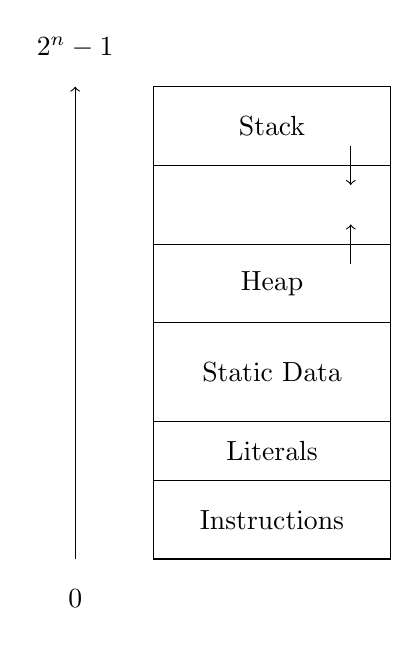
\begin{tikzpicture}
                            \draw
                            (0, 0) edge[->] (0, 6)
                            (1, 0) -- (4, 0) -- (4, 6) -- (1, 6) -- cycle
                            (1, 1) -- (4, 1)
                            (1, 1.75) -- (4, 1.75)
                            (1, 3) -- (4, 3)
                            (1, 4) -- (4, 4)
                            (1, 5) -- (4, 5)
                            (3.5, 5.25) edge[->] (3.5, 4.75)
                            (3.5, 3.75) edge[->] (3.5, 4.25);

                            \node[] () at (0, 6.5) {$2^n - 1$};
                            \node[] () at (0, -0.5) {0};

                            \node[] () at (2.5, 5.5) {Stack};
                            \node[] () at (2.5, 3.5) {Heap};
                            \node[] () at (2.5, 2.375) {Static Data};
                            \node[] () at (2.5, 1.375) {Literals};
                            \node[] () at (2.5, 0.5) {Instructions};
                        \end{tikzpicture}
                    \end{minipage} \
                    \begin{minipage}{0.725\textwidth}
                        \begin{itemize}
                            \itemsep0em
                            \item stack \hfill holds local variables, and procedure context
                                \subitem writable, not executable, and automatically managed by the compiler
                            \item heap (dynamic data) \hfill holds variables allocated with ~new~, or ~malloc~
                                \subitem writable, not executable, and managed by the programmer
                            \item static data \hfill ~static~ (including global) variables
                                \subitem writable, not executable, and initalized at start
                            \item literals \hfill such as ~"hello world"~, or ~143~
                                \subitem read-only, not executable, and initalized at start
                            \item instructions \hfill fairly self-explanatory
                                \subitem read-only, executable, and initalized at start
                        \end{itemize}
                    \end{minipage}
                \end{center}
                In the IA32 call stack, we have the bottom of the stack at the highest memory address, and the top of the stack at the lowest address. The stack pointer, ~\%esp~ holds the memory address of the top element, which is the lowest stack address. The stack generally grows downwards; therefore as we add things to the stack, the stack pointer gets lower, and as we take things off the stack - it gets higher.
                \medskip

                When we run the instruction ~pushl src~, we fetch the value from ~src~, decrement ~\%esp~ by 4 (4 bytes for a long), and store the value at the address given by ~\%esp~. On the other hand, when we run the corresponding ~\%popl dest~, we do reverse - we load the value from the address pointed by ~\%esp~, and write that value to ~dest~. ~\%esp~ is then incremented by 4. We should note that the value isn't actually removed - we're just removing the reference to it.
            \subsubsection*{Call Stacks}
                In general, a procedure call has a caller, and a callee. The caller first sets up arguments, and then calls the callee (which hands over control). The callee then creates its own local variables, runs some code, and then sets up the return value (to give back to the caller). It then cleans up its own local variables, and then gives control back to the caller. The caller then finds the return value from the callee. The following rules have to be observed;
                \begin{itemize}
                    \itemsep0em
                    \item callee must know where to find the arguments
                    \item callee must know where to find the return address
                    \item caller must know where to find the return value (hence know return address)
                    \item caller and callee need to run on the CPU, as they use the same registers; this also means they need to save some registers if it may be used by the other
                        \subitem this means that the caller has to save registers before setting up arguments, and then restore the registers after cleaning up the arguments, the same with the callee, but with local variables instead of arguments
                \end{itemize}
                This convention is called the \textbf{procedure call linkage}. Given a procedure call instruction ~call label~, we push the return address on the stack (which is the instruction immediately after the call), then we jump to ~label~. On the other hand, when we do a procedure return with ~ret~, we pop the return the address from the stack, and jump to that address.
                \medskip

                Actions that the \textcolor{blue}{caller} does are highlighted in blue, and actions that the \textcolor{violet}{callee} does are highlighted in violet;
                \begin{enumerate}[1.]
                    \itemsep0em
                    \item \textcolor{blue}{set parameters in order (registers, and stack)}
                    \item \textcolor{blue}{calls callee}
                    \item \textcolor{violet}{save registers on stack}
                    \item \textcolor{violet}{execute the body of method}
                    \item \textcolor{violet}{copy any results to ~\%eax~/~\%rax~}
                    \item \textcolor{violet}{restore registers from stack}
                    \item \textcolor{violet}{return to to caller}
                    \item \textcolor{blue}{remove parameters from stack}
                    \item \textcolor{blue}{use returned result}
                \end{enumerate}

                In this example, we put the address of the next instruction into ~\%eip~, push that value onto the stack, and then increment it by the arguments of ~call~ (we're using relative addressing). Note that ~0x8048590 = 0x8048553 + 0x000063d~. Note that it's an arbitrary number of instructions between ~0x8048590~, and ~0x8048591~, we're just using the latter to denote the ~ret~ instruction.
                \begin{lstlisting}
                    804854e:    e8 3d 06 00 00    call     8048b90 <main>
                    8048553:    50                pushl    %eax
                    .......
                    8048591:    c3                ret
                \end{lstlisting}
                \begin{center}
                    \begin{tabular}{r|l|l|l|l}
                        line & 1 & 2 & 3 & 4 \\
                        \hline
                        ~S: 0x110~ & & & & \\
                        ~S: 0x10c~ & & & & \\
                        ~S: 0x108~ & ~123~ & ~123~ & ~123~ & ~123~ \\
                        ~S: 0x104~ & & ~0x8048553~ & ~0x8048553~ &~0x8048553~ \\
                        ~\%esp~ & ~0x108~ & ~0x104~ & ~0x104~ & ~0x108~ \\
                        ~\%eip~ & ~0x804854e~ & ~0x8048590~ & ~0x8048591~ & ~8048553~ \\
                    \end{tabular}
                \end{center}
                By convention, we store the return value from a procedure in ~\%eax~. This is part of why it's important for the caller to save ~\%eax~, as this will be overwritten. If it doesn't fit in the 4 bytes, it's conventional just to return a pointer to the location where the return value is stored.
            \subsubsection*{Stack-based Languages}
                Languages thast support recursion are stack based languages, which requires code to be \textbf{re-entrant}, meaning that simultaneous instantiations of a single procedure is allowed. We need space to store the state of each instantiation, including arguments, local variables, and return pointers. The states are needed for a limited time, and the callee always returns before the caller does.
                \medskip

                In order to allow this, we need to create stack frames, which store the data previously mentioned. The space is allocated when the procedure is entered, and then deallocated on return. Stack frames are allocated by moving ~\%ebp~, and ~\%esp~. There's a good graphical example on the corresponding video, which would take me too long to draw out.
            \subsubsection*{IA32/Linux Stack Frame}
                We can construct the stack frame as such;
                \begin{center}
                    \begin{minipage}[t]{0.19\textwidth}
                        \begin{tabular}{|c|}
                            \hline
                            \\
                            \\
                            \\
                            \\
                            \\
                            \hline
                            \\
                            Arguments \\
                            \\
                            \hline
                            Return Address \\
                            \hline
                            Old ~\%ebp~ \\
                            \hline
                            \\
                            Saved \\
                            Registers \\
                            + Local \\
                            Variables \\
                            \\
                            \hline
                            Argument \\
                            Build \\
                            \hline
                        \end{tabular}
                    \end{minipage} \
                    \begin{minipage}{0.795\textwidth}
                        The initial space at the "bottom" of the stack (top of the diagram), is the memory used by the caller. The arguments are then put onto the stack, in the arguments section, and finally the return address, where the callee should return to, after completion. In the callee's frame, we also save the old pointer to the base of the caller's stack frame. Then there is more space for the callee's memory, and any arguments that might be used to call another function are put on the end.
                        \medskip

                        Revisiting the previous example for ~swap~, context is now provided for the offsets used.
                        \begin{center}
                            \begin{minipage}{0.4\textwidth}
                                \begin{lstlisting}
                                    swap:
                                        pushl %ebp
                                        movl  %esp, %ebp
                                        pushl %ebx

                                        movl 12(%ebp), %ecx
                                        movl 8(%ebp), %edx
                                        ...
                                \end{lstlisting}
                            \end{minipage} \
                            \begin{minipage}{0.58\textwidth}
                                \begin{center}
                                    \begin{tabular}{|r|c|}
                                        \hline
                                        offset from ~\%ebp~ & stack \\
                                        \hline
                                        & \\
                                        & \\
                                        & \\
                                        \hline
                                        12 & ~yp~ \\
                                        \hline
                                        8 & ~xp~ \\
                                        \hline
                                        4 & return addr \\
                                        \hline
                                        0 (~\%ebp~) & old ~\%ebp~ \\
                                        \hline
                                        -4 (~\%esp~) & old ~\&ebx~ \\
                                        \hline
                                    \end{tabular}
                                \end{center}
                            \end{minipage}
                        \end{center}
                    \end{minipage}
                \end{center}
\end{document}